\documentclass{article}

% if you need to pass options to natbib, use, e.g.:
%     \PassOptionsToPackage{numbers, compress}{natbib}
% before loading neurips_2023

% ready for submission
\usepackage[final]{neurips_2023}

% to avoid loading the natbib package, add option nonatbib:
%    \usepackage[nonatbib]{neurips_2023}

\usepackage[utf8]{inputenc} % allow utf-8 input
\usepackage[T1]{fontenc}    % use 8-bit T1 fonts
\usepackage{hyperref}       % hyperlinks
\usepackage{url}            % simple URL typesetting
\usepackage{booktabs}       % professional-quality tables
\usepackage{amsfonts}       % blackboard math symbols
\usepackage{amssymb}        % for math symbols like \leq and \geq
\usepackage{nicefrac}       % compact symbols for 1/2, etc.
\usepackage{microtype}      % microtypography
\usepackage{xcolor}         % colors
\usepackage{graphicx}       % for including figures
\usepackage{subcaption}     % for subfigures
\usepackage{float}          % for H placement option


\title{MLPC 2025: Sound Event Detection Data Exploration}

\author{
  Team Imported \AND
  Lóránd Heidrich
  \And
  Mark Sere
  \And 
  Gergely Terényi
  \And 
  Diego Caparros Vaquer
}

\begin{document}

\maketitle
\section{Statement of contributions}
Diego Caparros Vaquer led the case study and report. Lóránd Heidrich analyzed annotation quality and created presentation slides. Mark Sere focused on audio features, clustering, and the data pipeline. Gergely Terényi worked on text features, clustering, and the conclusion.

\begin{abstract}
This report analyzes the MLPC 2025 Sound Event Detection dataset, focusing on annotation quality, audio features, and text patterns. It evaluates temporal precision, textual similarity, and audio features, highlighting challenges and biases to inform future model development.
\end{abstract}

\section{Introduction}

This report analyzes the MLPC 2025 Sound Event Detection dataset from Kepler Intelligent Audio Labs (KIAL), consisting of 9,026 audio files (15-30s) and 35,826 textual annotations from 330 students. It examines annotation quality, audio, and text features to identify key dataset characteristics and challenges for sound event detection training.

\section{Case Study}
\label{sec:case_study}

\begin{table}[H]
  \caption{Conclusions}
  \label{tab:text_similarity}
  \centering
  \scalebox{0.5}{\begin{tabular}{c|c|c}
    \toprule
    Aspect & Audio 1 (407115.mp3) & Audio 2 (352781.mp3) \\
    \midrule
    Temporal Annotation & General agreement, differences in granularity. & Strong alignment across annotators; treated as a continuous ambient scene. \\
    Textual Annotation & Annotators 2 \& 3 vary in wording and include unique sounds. & Shared themes of muffled speech and indoor ambience, with slight variations. \\
    Metadata Alignment & Adds foreground sounds not in metadata & Near-perfect alignment. \\
    Task Compliance & Annotations follow temporal rules and provide detailed, context-specific descriptions. & Annotations follow temporal rules and provide detailed, context-specific descriptions.\\
    \bottomrule
  \end{tabular}}
\end{table}

\section{Annotation Quality}
\label{sec:annotation_quality}

\subsection{Temporal Annotation Precision}

Temporal annotation precision was assessed by comparing onset/offset timings of overlapping segments from different annotators. Metrics included Euclidean distance, and onset/offset differences.

\begin{figure}[H]
  \centering
  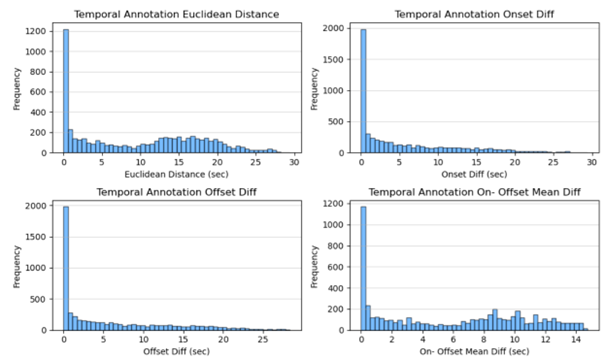
\includegraphics[width=0.3\textwidth]{figures/annotation_quality/temporal_annotation_differences.png}
  \caption{Temporal Annotation Differences}
  \label{fig:temporal_diff}
\end{figure}

Results show a strong agreement near 0s (indicating shared timing), with all distributions positively skewed. Onset/offset differences taper off before 5s, while Euclidean distance reveals a secondary peak around 12–20s—suggesting localized disagreement.

Overall, temporal precision is high, though some segments remain ambiguous and harder to segment accurately.

\subsection{Text Annotation Similarity}

\begin{figure}[H]
  \centering
  \begin{minipage}{0.4\textwidth}
    \centering
    \begin{table}[H]
      \caption{Similarity of Overlapping Text Annotations Stats}
      \label{tab:text_similarity_1}
      \scalebox{0.4}{\begin{tabular}{lc}
        \toprule
        Metric & Value \\
        \midrule
        Range & -0.29 -- 0.75 \\
        Mean & 0.088 \\
        Median & 0.072 \\
        \bottomrule
      \end{tabular}}
    \end{table}
  \end{minipage} \hfill
  \begin{minipage}{0.4\textwidth}
    \centering
    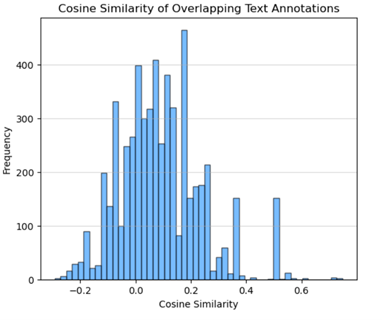
\includegraphics[width=0.5\textwidth]{figures/annotation_quality/similarity_of_overlapping_text_annotations.png}
    \caption{Similarity of Overlapping Text Annotations}
    \label{fig:text_similarity_2}
  \end{minipage}
\end{figure}

Most overlapping annotations show low textual similarity. Cosine similarity ranges from –0.29 to 0.75, with a mean of 0.088 and median of 0.072, indicating varied wording or focus among annotators (see Table~\ref{tab:text_similarity}). The histogram confirms weak agreement, with most values clustered between 0 and 0.2.

\subsection{Annotation Distribution}

\begin{figure}[H]
  \centering
  \begin{minipage}{0.32\textwidth}
    \centering
    \begin{table}[H]
      \caption{Per File Measures}
      \label{tab:per_file}
      \scalebox{0.5}{\begin{tabular}{lcc}
        \toprule
        & Annotations/File & Distinct Sound Events/File \\
        \midrule
        Total Unique Files & 9026 & 9026 \\
        Total Annotations & 35826 & 35826 \\
        Mean & 3.9692 & 2.4253 \\
        Median & 2 & 2 \\
        STD & 4.4254 & 1.9063 \\
        Min & 1 & 1 \\
        Q1 & 1 & 1 \\
        Q2 & 2 & 2 \\
        Q3 & 5 & 3 \\
        Max & 96 & 27 \\
        \bottomrule
      \end{tabular}}
    \end{table}
  \end{minipage} \hfill
  \begin{minipage}{0.2\textwidth}
    \centering
    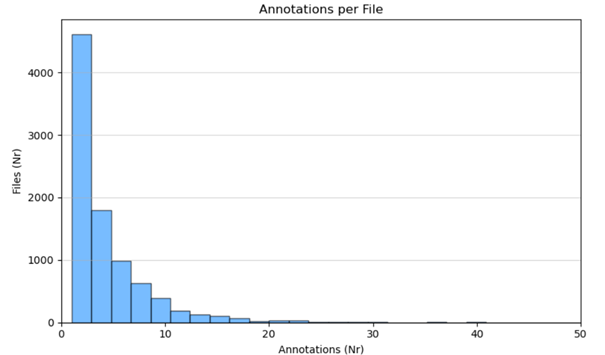
\includegraphics[width=\textwidth]{figures/annotation_quality/annotations_per_file.png}
    \caption{Annotations Per File}
    \label{fig:annotations_per_file}
  \end{minipage} \hfill
  \begin{minipage}{0.2\textwidth}
    \centering
    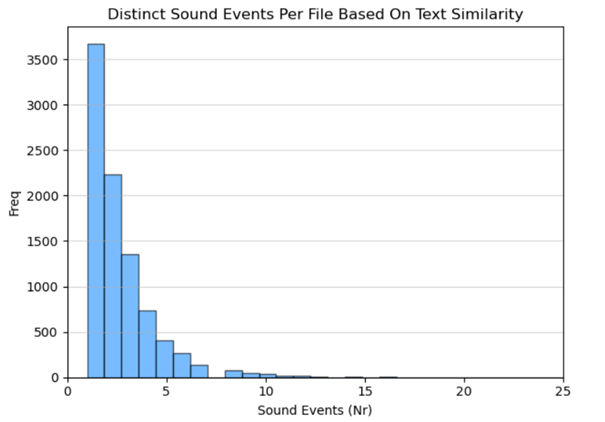
\includegraphics[width=\textwidth]{figures/annotation_quality/distinct_sound_events_per_file.png}
    \caption{Distinct Sound Events Per File}
    \label{fig:distinct_sound_events_per_file}
  \end{minipage}
\end{figure}

Table~\ref{tab:per_file} shows the statistics for annotations per file and distinct sound events per file. The dataset has a mean of approximately 4 annotations per file with a median of 2, indicating a positively skewed distribution. The maximum number of annotations for a single file is 96, which is significantly higher than the average.

\begin{table}[H]
  \caption{Text Annotation Detail}
  \label{tab:text_detail}
  \centering
  \scalebox{0.5}{\begin{tabular}{lc}
    \toprule
    Metric & Value \\
    \midrule
    Total annotations & 35826 \\
    Mean word count & 7.4874 \\
    Median & 7 \\
    STD & 4.6315 \\
    Min & 1 \\
    Q1 & 4 \\
    Q2 & 7 \\
    Q3 & 9 \\
    Max & 88 \\
    \bottomrule
  \end{tabular}}
\end{table}

The annotations have an average word count of 7.85 words. The histogram in Figure~\ref{fig:word_count_avg_word_count_avg_duration} shows a concentration between 5-10 words (a reasonable amount considering the annotation guidelines), however some annotators averaged over 20 words. The positive skew is indicative of this high variability.

\begin{figure}[h]
    \centering
    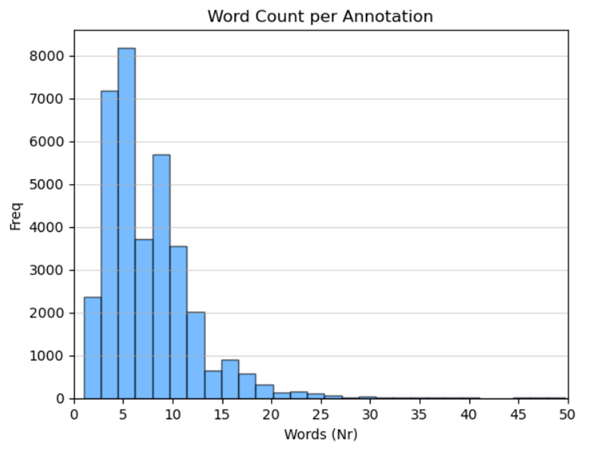
\includegraphics[width=0.3\linewidth]{figures/annotation_quality/word_count_per_annotation.png}
    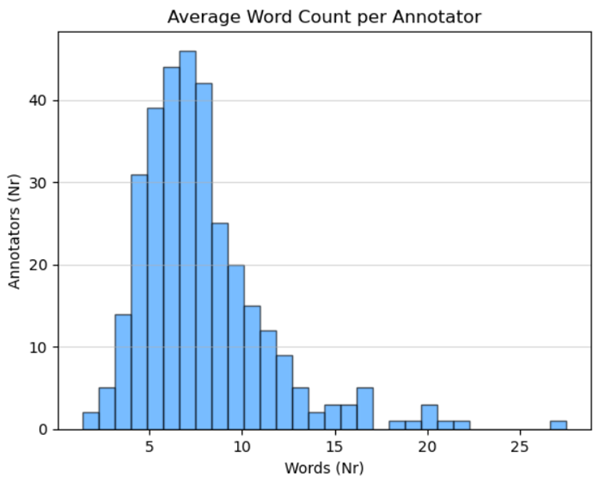
\includegraphics[width=0.3\textwidth]{figures/annotation_quality/average_word_count_per_annotator.png}
    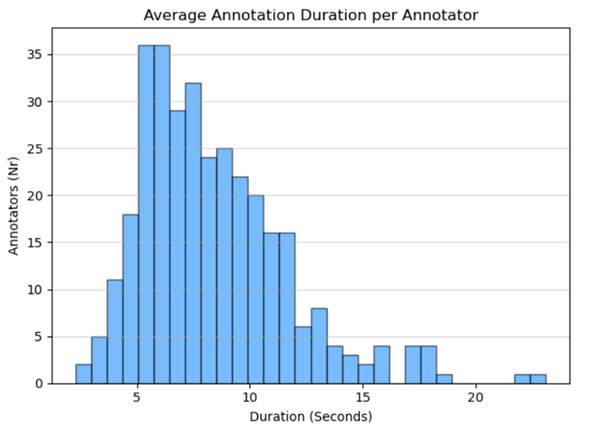
\includegraphics[width=0.3\textwidth]{figures/annotation_quality/average_annotation_duration_per_annotator.png}
    \caption{Word Count Per Annotation and Average Word Count Per Annotator, respectively} \label{fig:word_count_avg_word_count_avg_duration}
\end{figure}

Most events were marked in the 5–10s range, with an average duration of 8.38s. A long-tail distribution shows some annotators marked events over 20s, reflecting differing perceptions. The standard deviation of 3.31s suggests moderate variation.

\subsection{Inconsistencies and Quality Issues}

Annotation duration, word count, and spelling errors were the indicators used to detect inconsistencies, outliers, and poor-quality annotations. Outlier thresholds were set both by IQR and explicit selection, following best practices and empirical testing.

\begin{figure}[H]
  \centering
  \begin{minipage}{0.45\textwidth} % Adjusted width for the first table
    \centering
    \begin{table}[H]
      \caption{Duration and Word Count Metrics}
      \label{tab:duration_word}
      \centering
      \scalebox{0.5}{\begin{tabular}{lcc}
        \toprule
        & Duration & Word Count \\
        \midrule
        Count & 35826 & 35826 \\
        Mean & 7.3139 & 7.4874 \\
        Median & 2.6609 & 7 \\
        STD & 8.7611 & 4.6315 \\
        Min & 0 & 1 \\
        1\% & 0.1323 & 2 \\
        5\% & 0.2721 & 2 \\
        Q1 & 0.9712 & 4 \\
        Q3 & 12.6279 & 9 \\
        95\% & 26.1306 & - \\
        99\% & 29.2635 & - \\
        Max & 30.0447 & 88 \\
        IQR & 11.6567 & 5 \\
        IQR lower threshold & -16.5138 & -3.5 \\
        IQR upper threshold & 30.113 & - \\
        \bottomrule
      \end{tabular}}
    \end{table}
  \end{minipage}  
  \begin{minipage}{0.45\textwidth} % Adjusted width for the second table
    \centering
    \begin{table}[H]
    \captionsetup{justification=centering}
      \caption{Duration Outcomes}
      \label{tab:duration_outcomes}
      \centering
      \scalebox{0.5}{\begin{tabular}{lccc}
        \toprule
        & IQR & 99\% & 95\% \\
        \midrule
        Text too short (annotations) & 0 & 355 & 1792 \\
        Text too long (annotations) & 0 & 359 & 1792 \\
        Text too short (\%) & 0\% & 0.9909\% & 5.0020\% \\
        Text too long (\%) & 0\% & 1.0021\% & 5.0020\% \\
        \bottomrule
      \end{tabular}}
    \end{table}
  \end{minipage}
\end{figure}

Event duration markers found no IQR lower outliers, therefore the central range is wide and tolerant. Explicit 1\%/99\% thresholds flagged 0.99\%/1\% of annotations respectively, while 5\%/95\% thresholds flagged 5\% each, showing that most annotations are reasonable, with few consistent outliers. Text length analysis found no IQR-based outliers, and only 0.94\% fell below the 5th percentile. While there were no zero-word annotations, many were short: 335 had one word, 2024 had two, and 3146 had three. Overall, 26.62\% (9537 annotations) were under five words—below the guideline's ideal length—suggesting a substantial portion may lack descriptive detail.

\begin{table}[H]
  \caption{Word Count Outcomes}
  \label{tab:word_outcomes}
  \centering
  \scalebox{0.5}{\begin{tabular}{lcccc}
    \toprule
    & 1\% & 5\% & IQR Lower & Explicit 5 \\
    \midrule
    Word threshold & 2 & 2 & -3.5 & 5 \\
    Annotation Count & 335 & 335 & 0 & 9537 \\
    Annotation Proportion & 0.9351\% & 0.9351\% & 0\% & 26.6203\% \\
    \bottomrule
  \end{tabular}}
\end{table}

Spelling, assessed via pyspellchecker, showed 49.56\% of annotations error-free. About 32.3\% had one error, 15\% had 2–3, and 3\% had 4 or more.

Using combined quality flags—extreme durations (<1\% or >99\%), very short text ($\leq$ 2 words), and high misspell count ($\geq$3)—15.25\% of annotations were marked low quality. With a 5\% duration threshold, this rose to 22.14\%.

After filtering for files with multiple annotators, each annotator averaged 4.5 files (STD = 2.59), with a range of 1–27, reflecting a small, skewed dataset that may limit generalizability.

\subsubsection{Proposed Solution for Inconsistencies}

Spelling errors, word count, and duration outliers can be programmatically flagged for review. A random sample of these flagged files can help determine if reannotation is needed, in which case the files can be reassigned to their original annotators.

\section{Audio Features}
\label{sec:audio_features}

\subsection{Feature Selection and Dimensionality Reduction}

\begin{figure}[H]
  \centering
  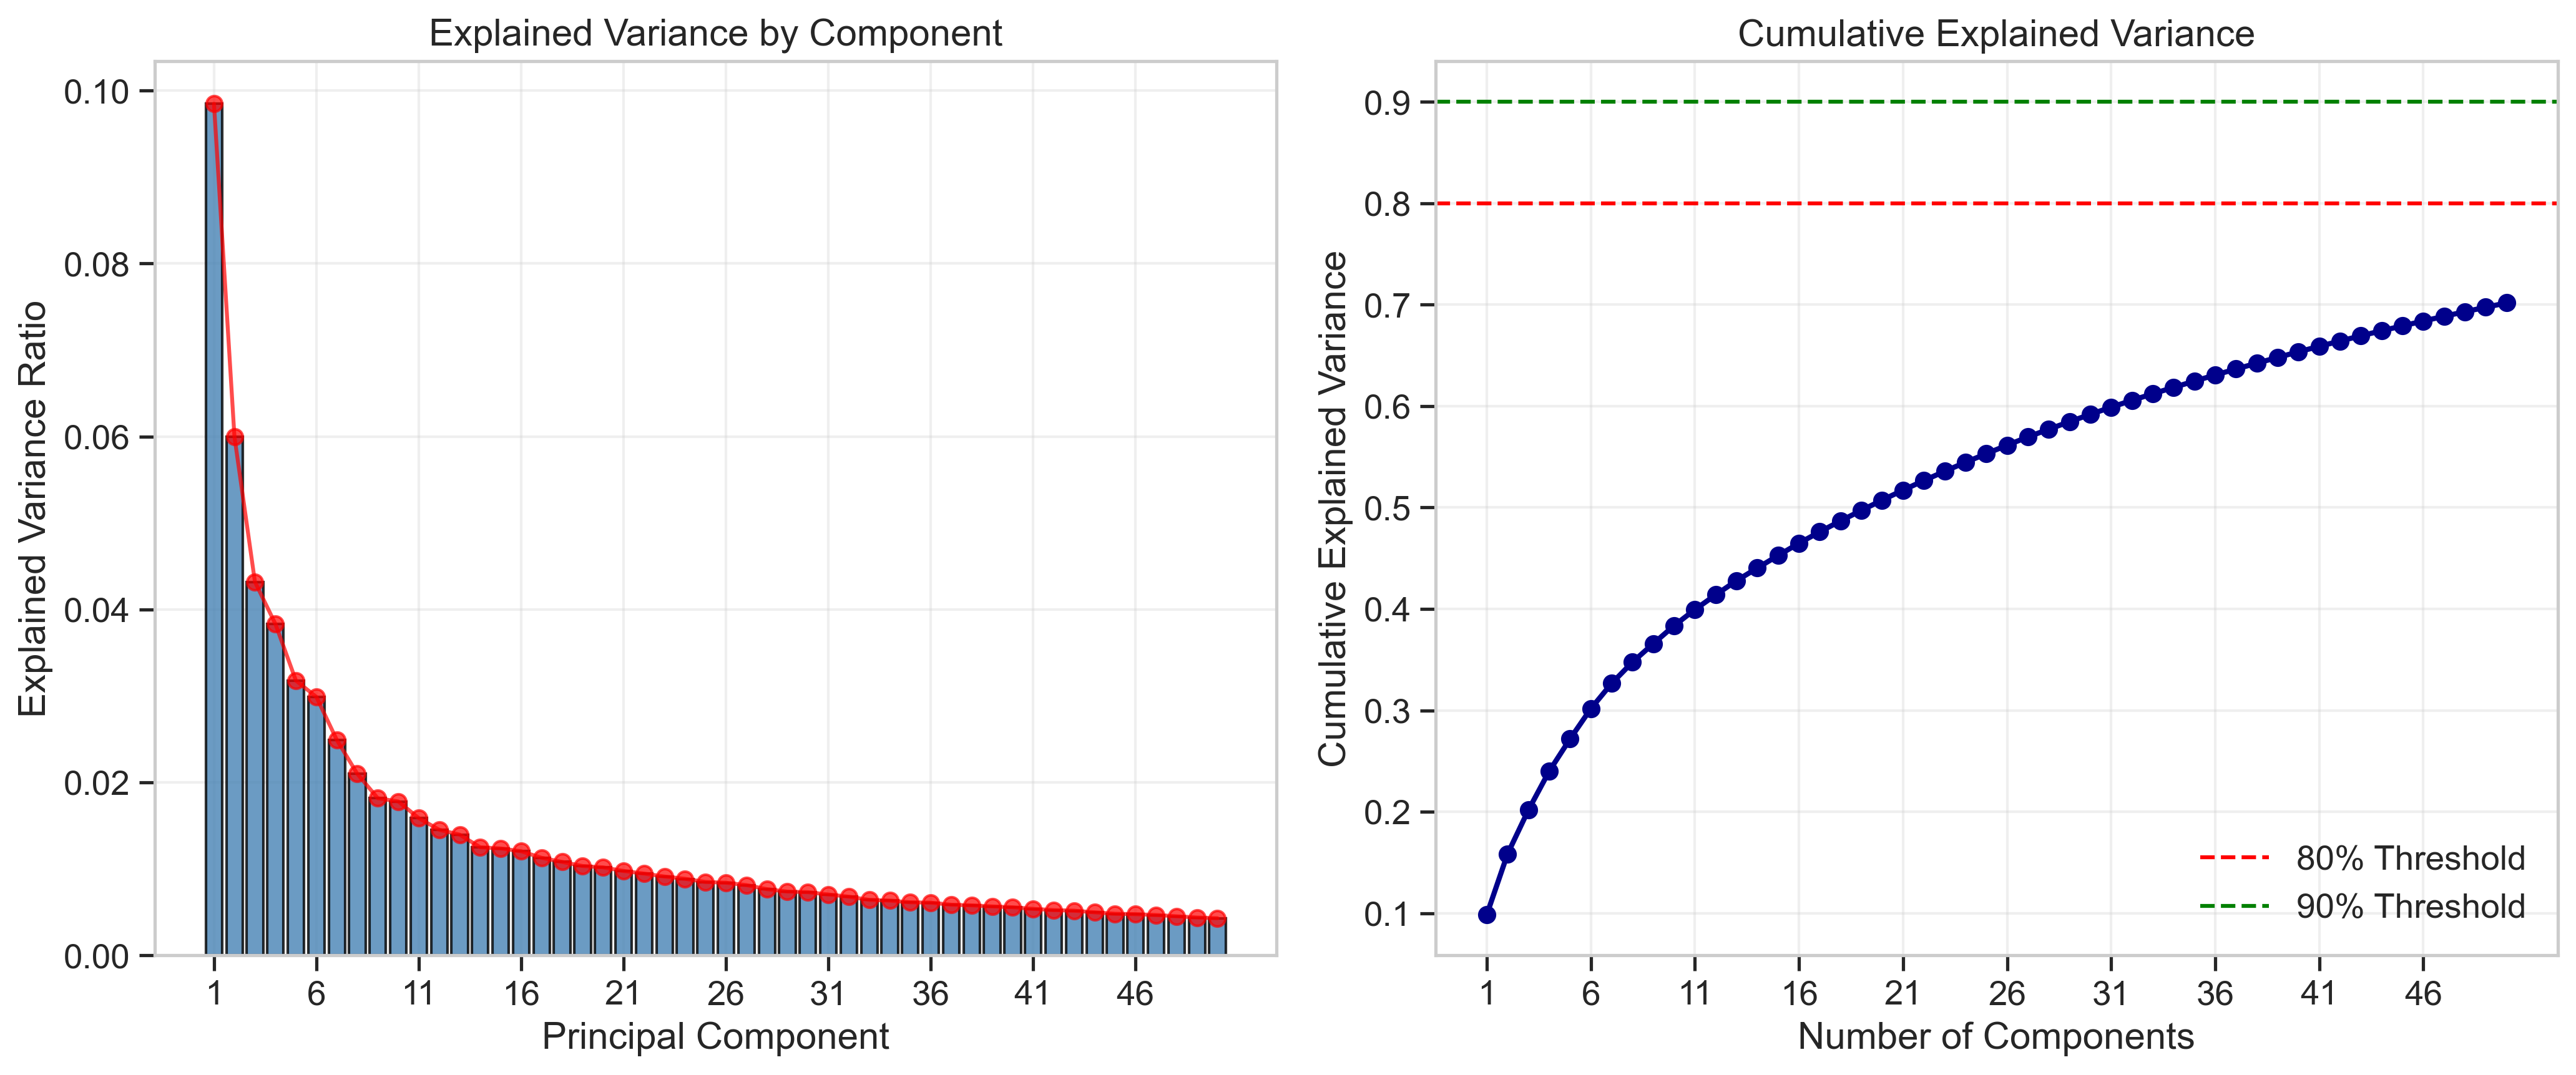
\includegraphics[width=0.3\textwidth]{figures/audio_features/pca_explained_variance.png}
  \caption{Explained variance by PCA components. Left: Individual variance contribution of each component. Right: Cumulative explained variance with 80\% and 90\% thresholds marked.}
  \label{fig:pca_variance}
\end{figure}

Analysis of the cumulative explained variance revealed that 82 principal components are sufficient to explain 80\% of the variance and 146 components are needed to explain 90\% of the variance. This represents a significant dimensionality reduction (from 942 to 82 dimensions, or 91.3\% reduction) while maintaining most of the information content. The reduced feature set was used for subsequent clustering analysis.

\subsection{Feature Importance}

To understand which features contribute most to the principal components, the feature loadings for the top three components were analyzed.

\begin{figure}[H]
  \centering
  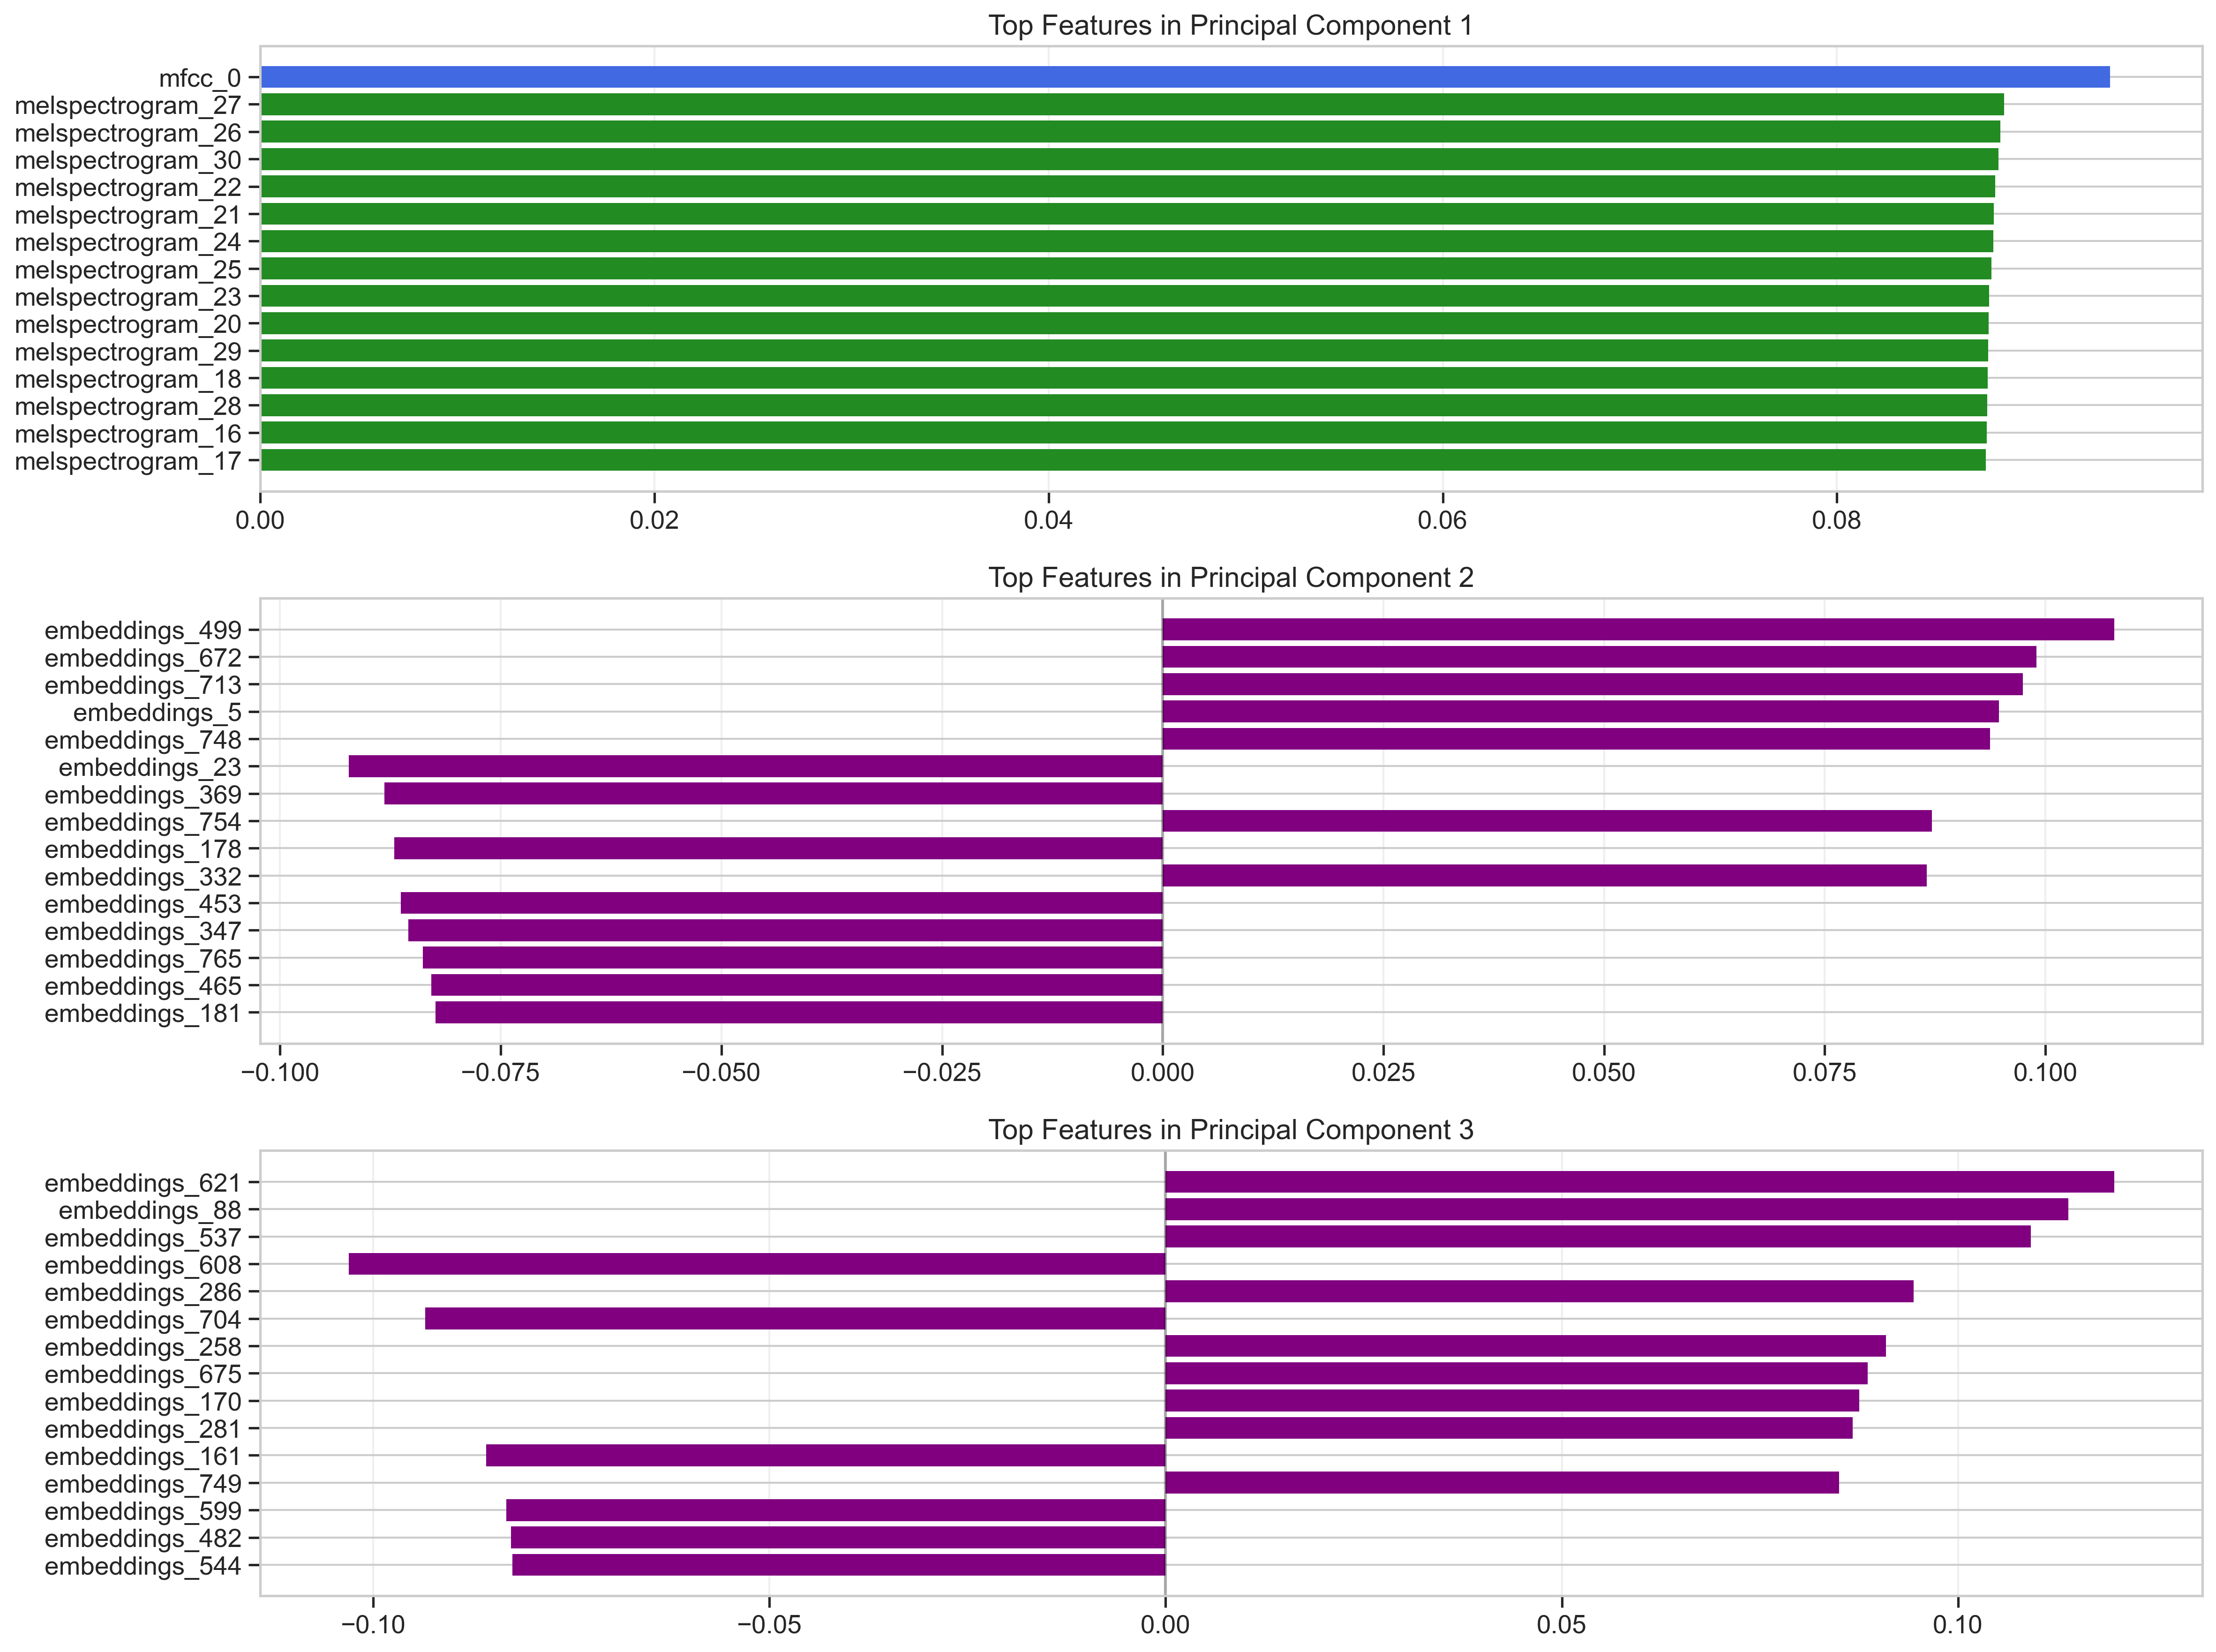
\includegraphics[width=0.3\textwidth]{figures/audio_features/feature_importance.png}
  \caption{Top 15 features contributing to the first three principal components, showing the relative importance of different feature types.}
  \label{fig:feature_importance}
\end{figure}

The analysis revealed:
\begin{itemize}
    \item \textbf{First principal component}: Driven by Mel spectrogram features, especially MFCC\_0, highlighting energy distribution as key for distinguishing audio.
    \item \textbf{Second and third principal components}: Shaped by neural network embeddings, likely capturing higher-level semantic audio features.
\end{itemize}

Across the top three components, the most important feature types were: Embeddings: 30 occurrences, Mel spectrogram features: 14 occurrences, MFCCs: 1 occurrence

This suggests that while traditional spectral features like MFCCs are valuable, the learned embeddings capture additional information that contributes significantly to the variance in the data.

\subsection{Clustering Analysis}

K-means clustering was applied to the dimensionally-reduced feature vectors to identify natural groupings in the audio data. To determine the optimal number of clusters, silhouette scores were calculated for different values of k.

\begin{figure}[H]
  \centering
  \begin{minipage}{0.45\textwidth} % Adjusted width for the first image
    \centering
    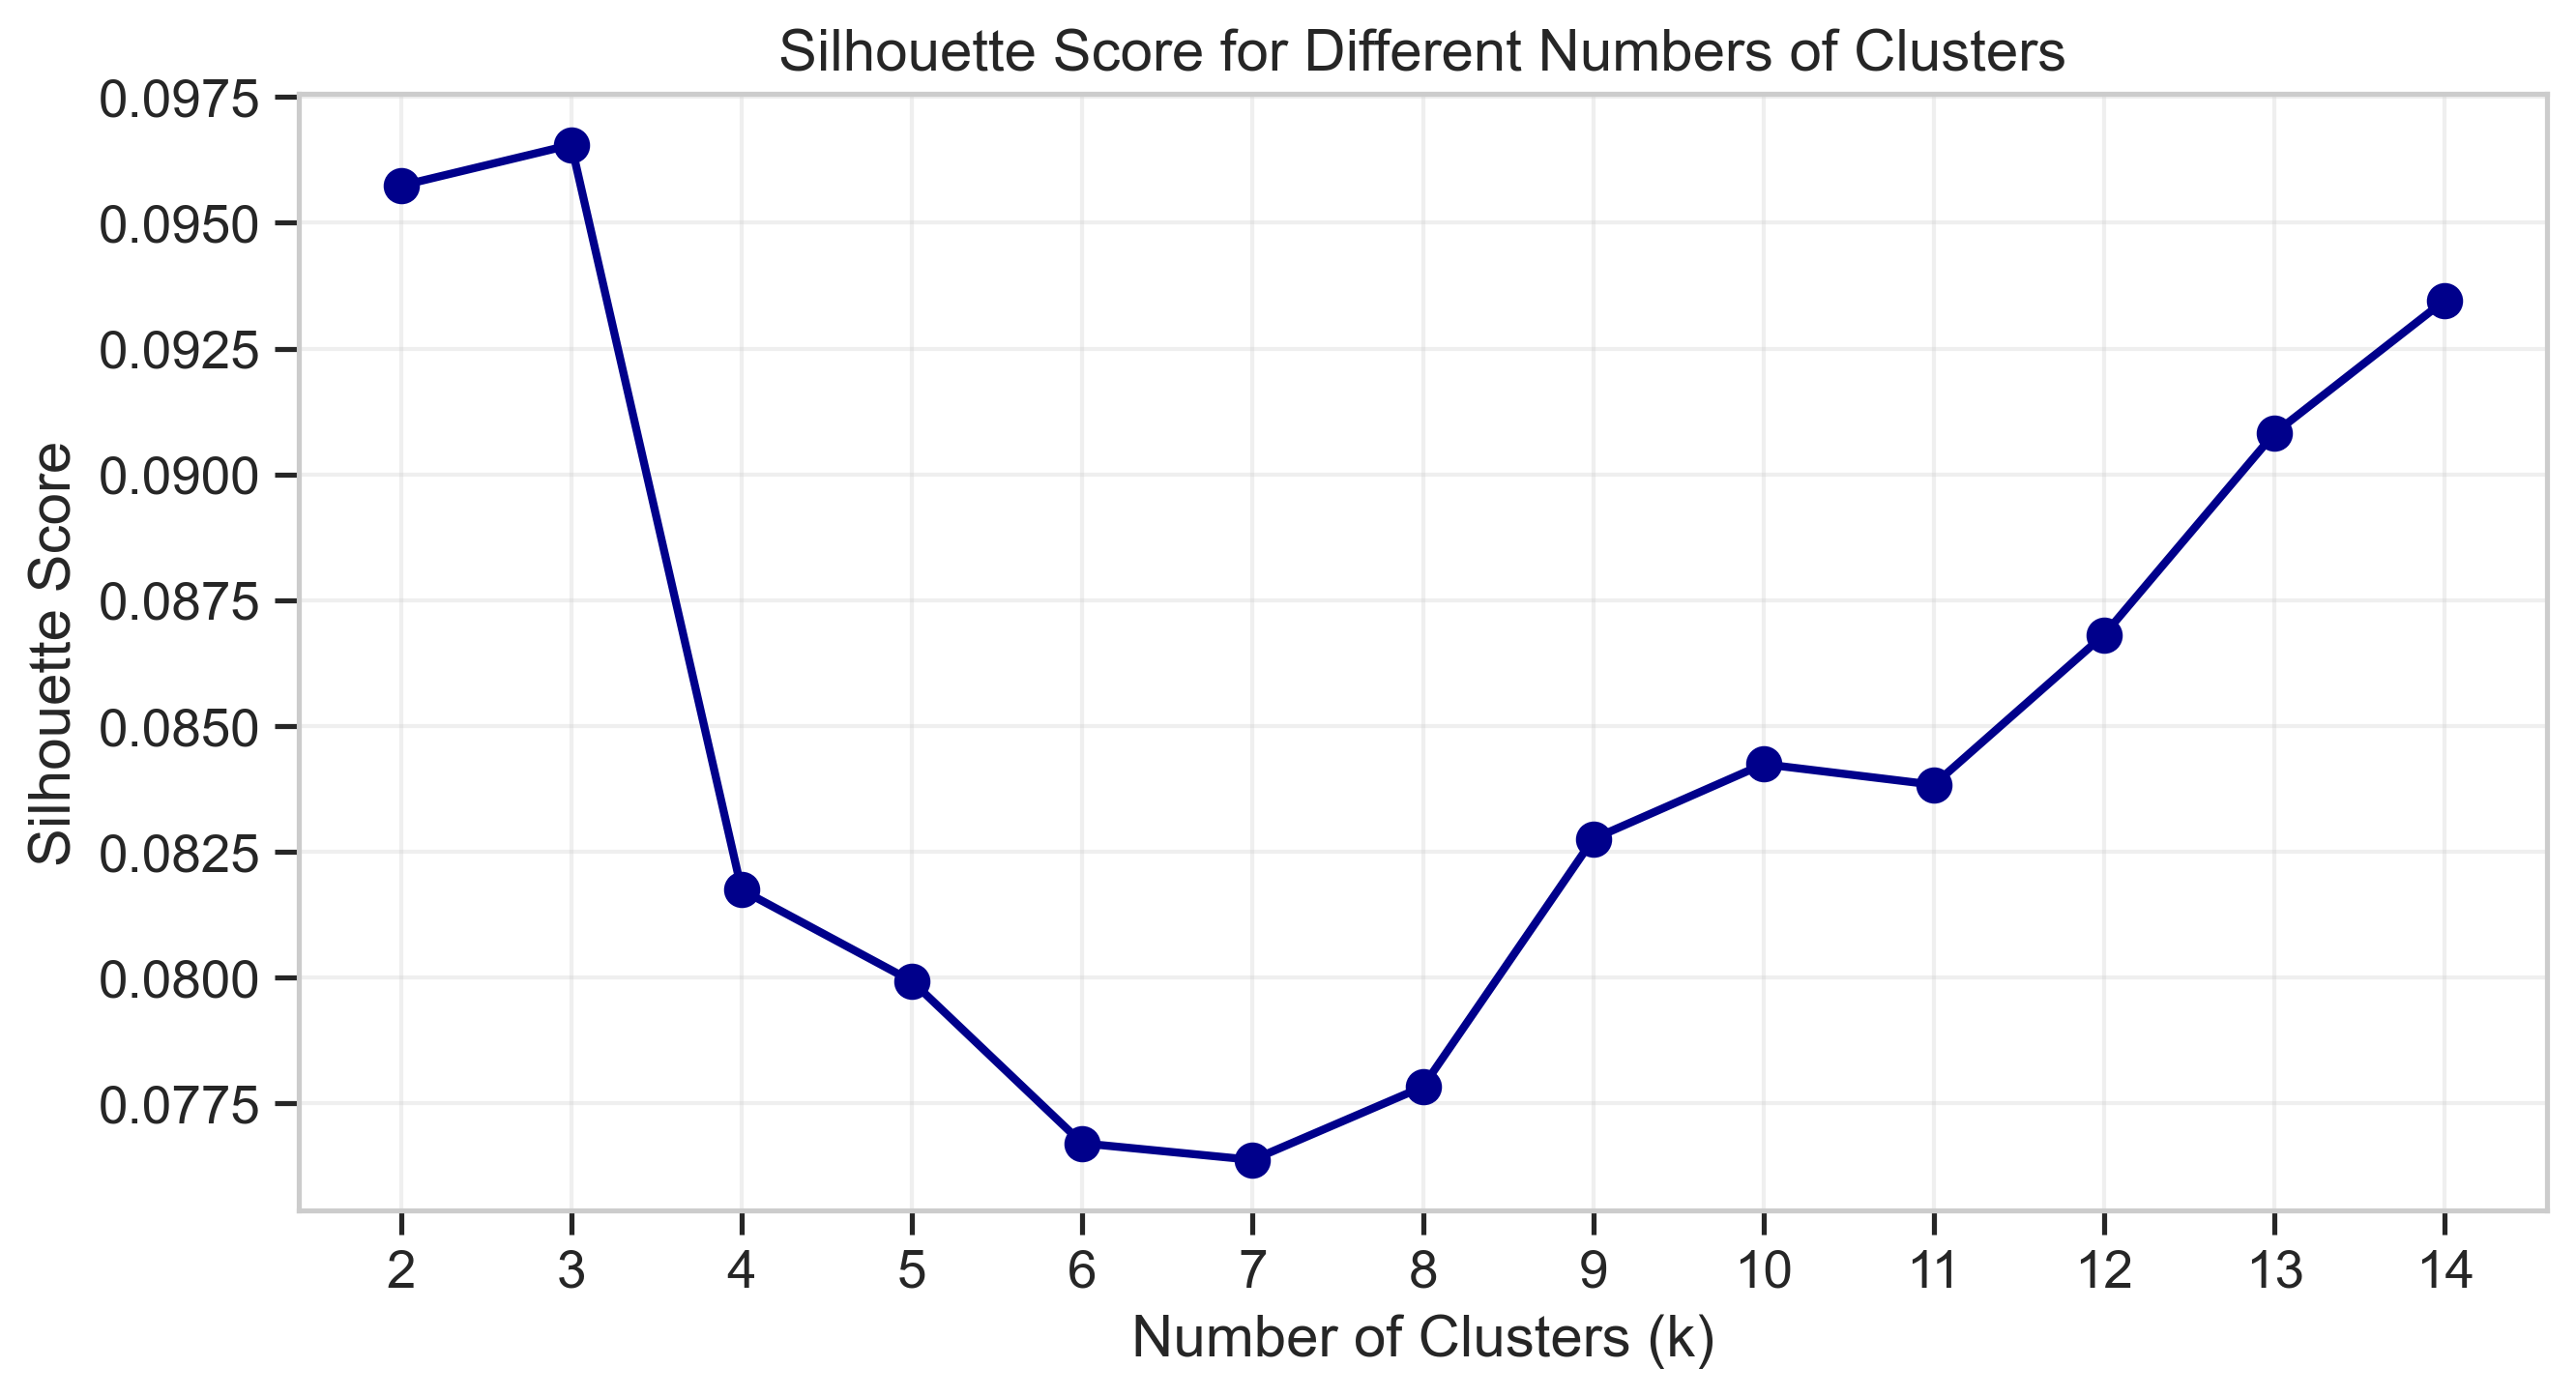
\includegraphics[width=0.8\linewidth]{figures/audio_features/silhouette_scores.png}
    \caption{Silhouette scores for different numbers of clusters (k), showing that k=3 provides the best cluster separation.}
    \label{fig:silhouette}
  \end{minipage} \hspace{0.05\textwidth} % Horizontal space between the images
  \begin{minipage}{0.45\textwidth} % Adjusted width for the second image
    \centering
    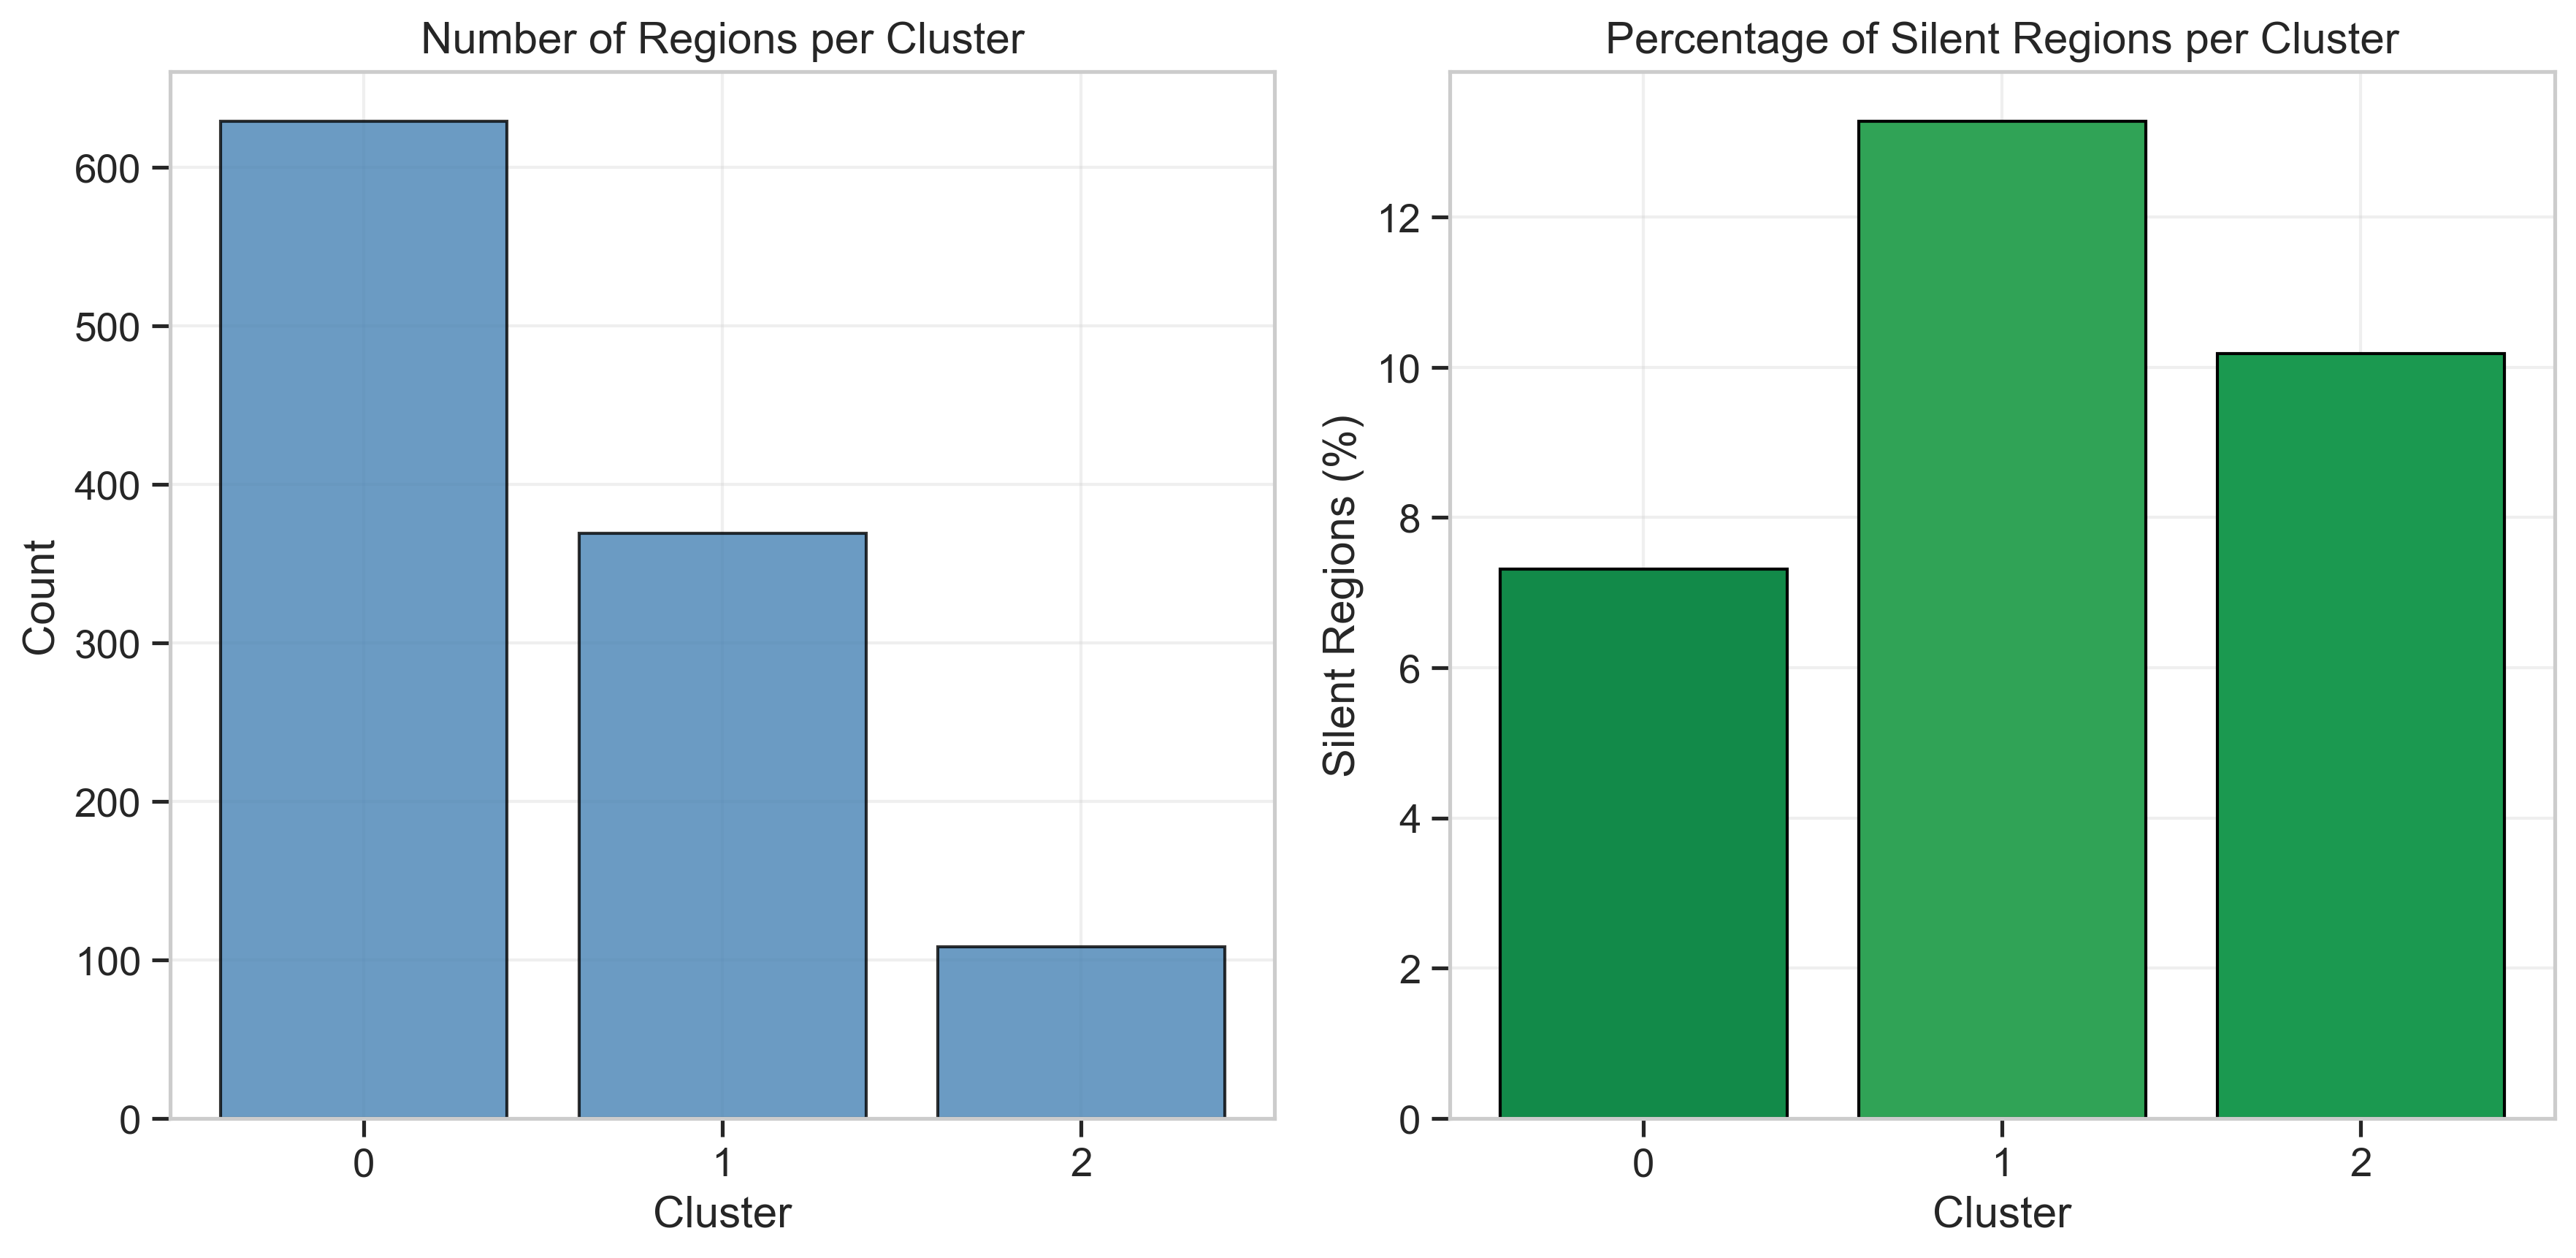
\includegraphics[width=0.8\linewidth]{figures/audio_features/cluster_composition.png}
    \caption{Left: Number of audio regions in each cluster. Right: Percentage of silent regions in each cluster.}
    \label{fig:cluster_comp}
  \end{minipage}
\end{figure}

The silhouette analysis indicated that 3 clusters provided the optimal balance between cluster separation and cohesion. The dataset was subsequently partitioned into these three clusters.

\subsection{Cluster Characteristics}

Analysis of the three clusters revealed distinct audio characteristics:

\begin{table}[H]
  \caption{Characteristics of the three audio feature clusters}
  \label{tab:cluster_chars}
  \centering
  \scalebox{0.5}{\begin{tabular}{p{1.5cm}p{3cm}p{4cm}p{3cm}}
    \toprule
    \textbf{Cluster} & \textbf{Size \& Silent \%} & \textbf{Common Annotations} & \textbf{Audio Characteristics} \\
    \midrule
    Cluster 0 & 629 regions (56.9\%) \newline 7.3\% silent regions & Beeps, cat meows, pedestrian crossing sounds, metallic impacts & High embedding values, predominantly sharp, distinct sounds \\
    \midrule
    Cluster 1 & 369 regions (33.4\%) \newline 13.3\% silent regions & Insect buzzing, dog barking, bass drums, human vocalizations & Low embedding values, more sustained sounds with less tonal clarity \\
    \midrule
    Cluster 2 & 108 regions (9.8\%) \newline 10.2\% silent regions & Hihat sounds, guitar playing, rhythmic claps, alarm-like sounds & High embedding values, musical and rhythmic sounds \\
    \bottomrule
  \end{tabular}}
\end{table}

Interestingly, silent regions were distributed across all three clusters rather than being concentrated in a single cluster. Cluster 1 had the highest percentage of silent regions (13.3\%), suggesting that this cluster might represent lower-energy or background sounds.

\subsection{Visualization of Audio Feature Space}

\begin{figure}[H]
  \centering
  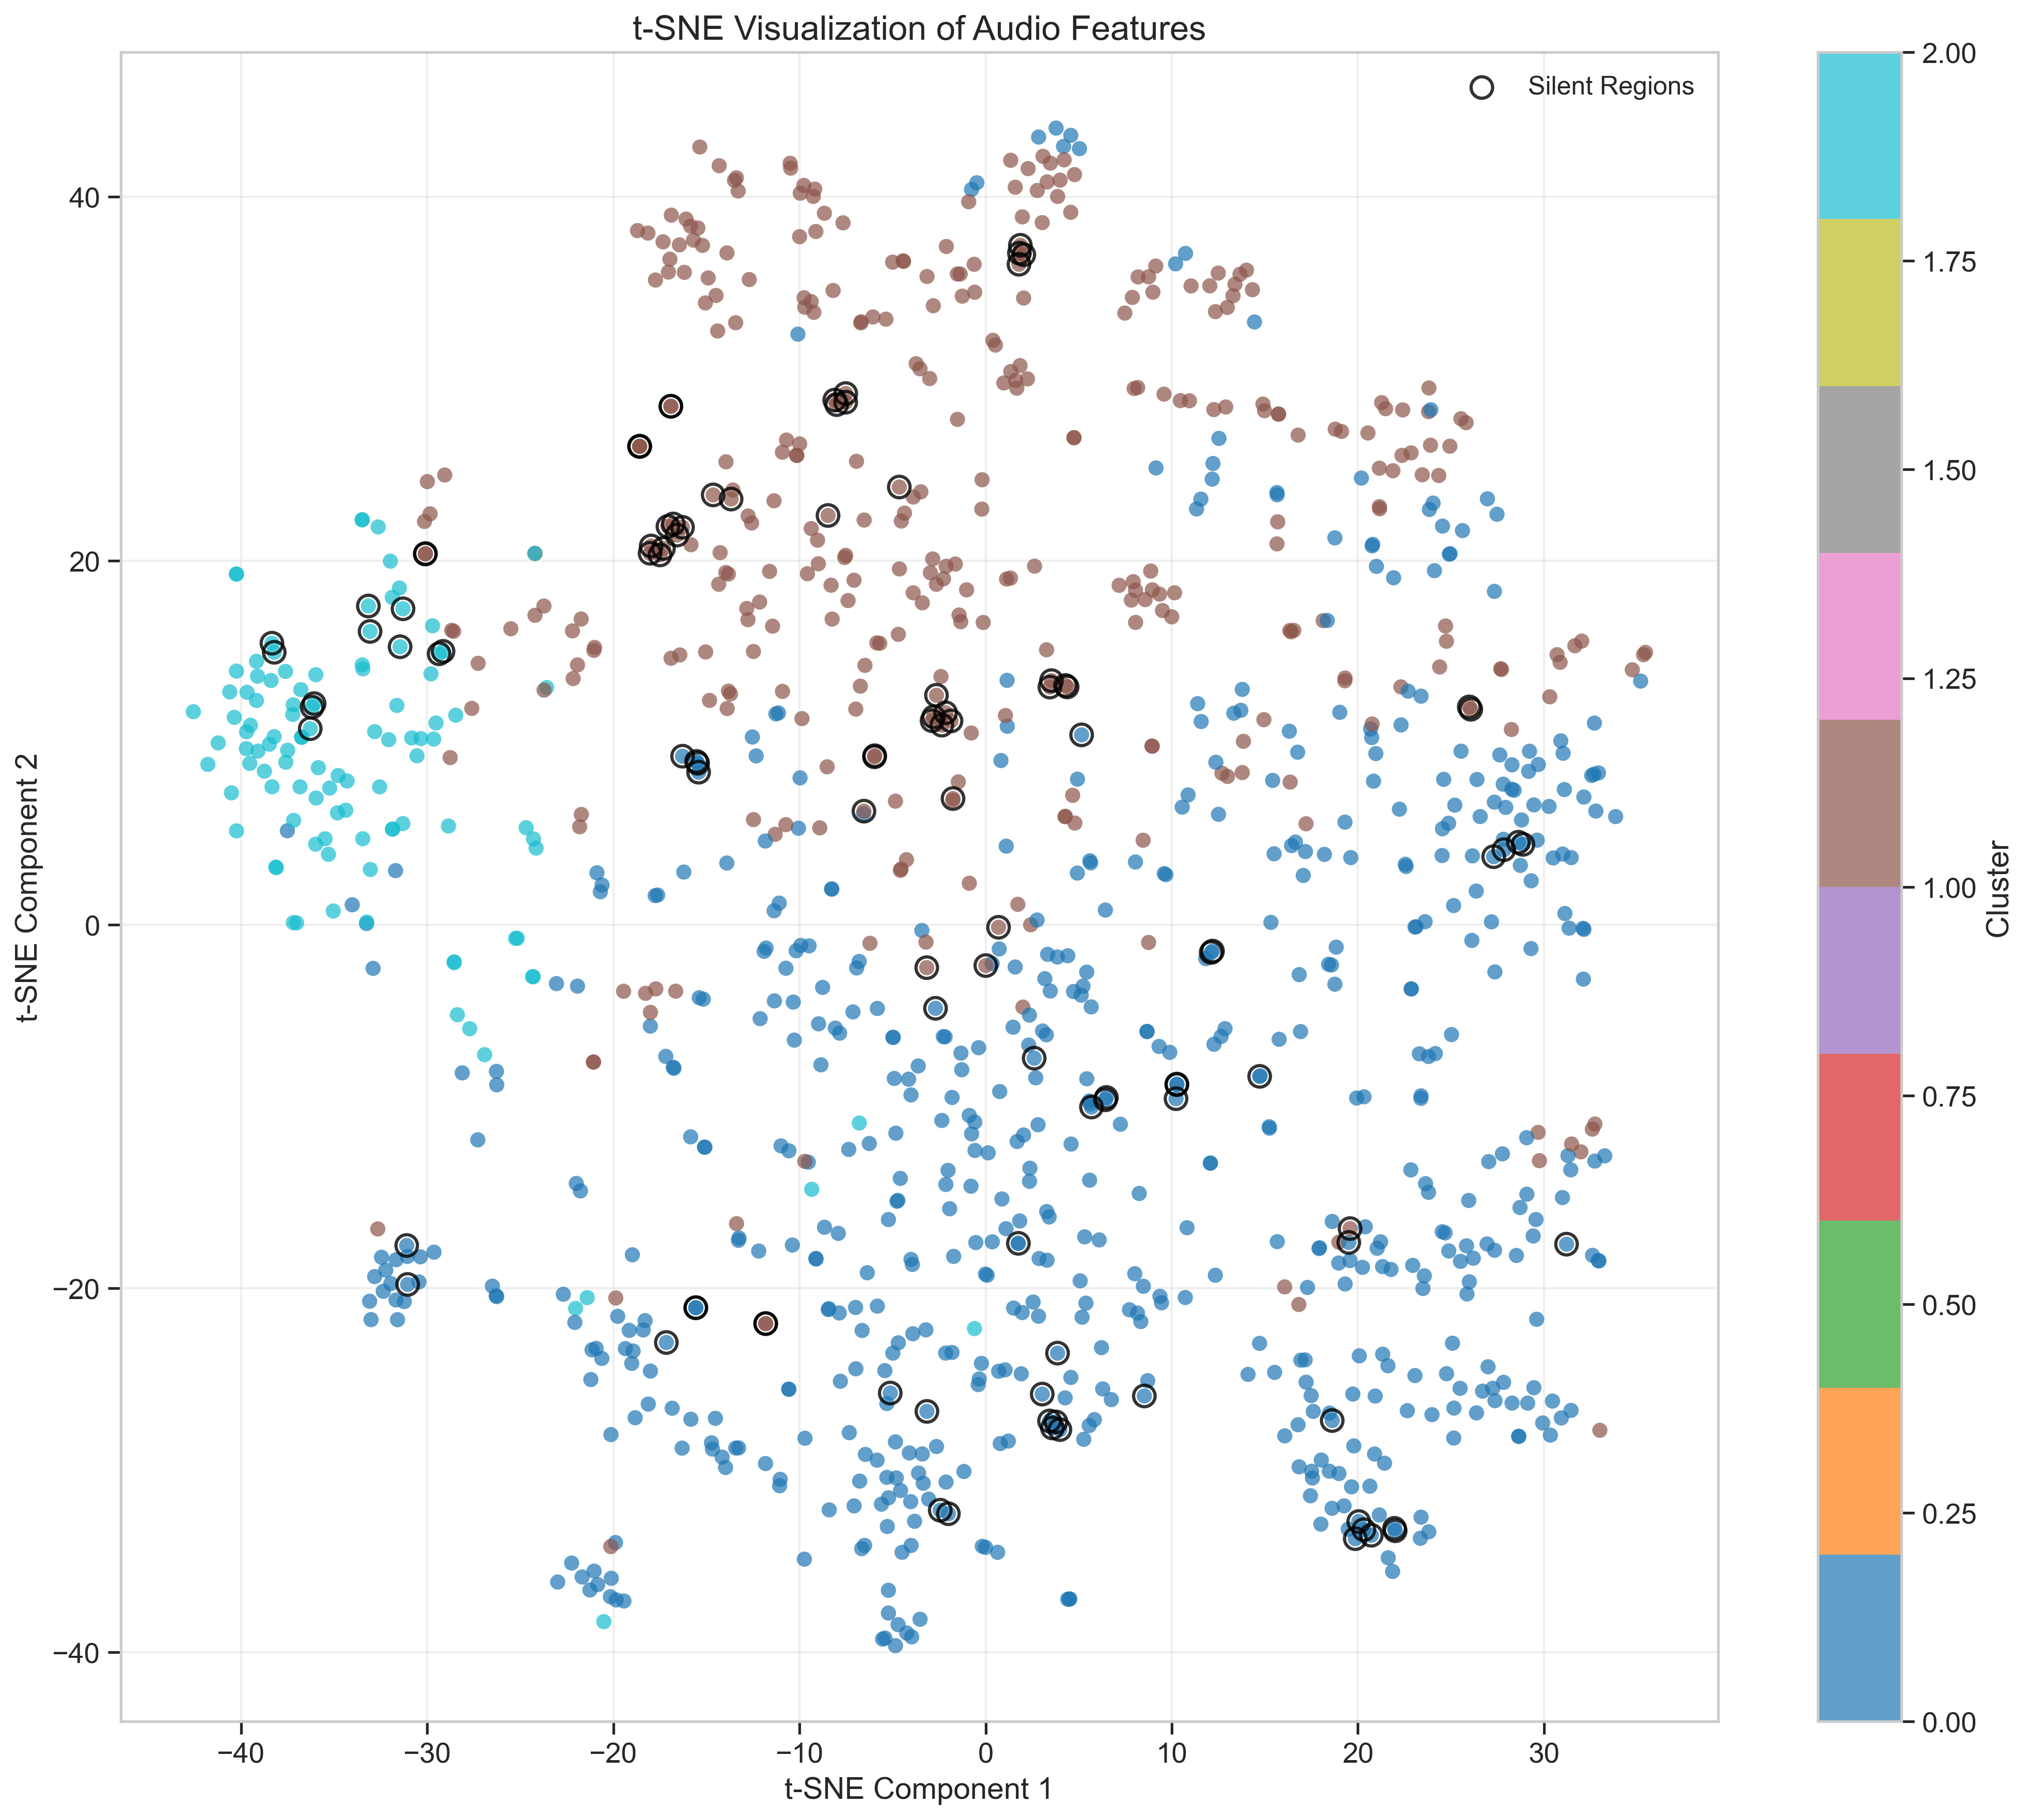
\includegraphics[width=0.3\textwidth]{figures/audio_features/tsne_visualization.png}
  \caption{t-SNE visualization of audio features colored by cluster assignment, though boundaries are often blurred with overlapping sound types. Silent regions are highlighted with black circles.}
  \label{fig:tsne}
\end{figure}

\section{Text Features}
\label{sec:text_features}
\subsection{Clustering text features, meaningful clusters}
\begin{figure}[H]
  \centering
  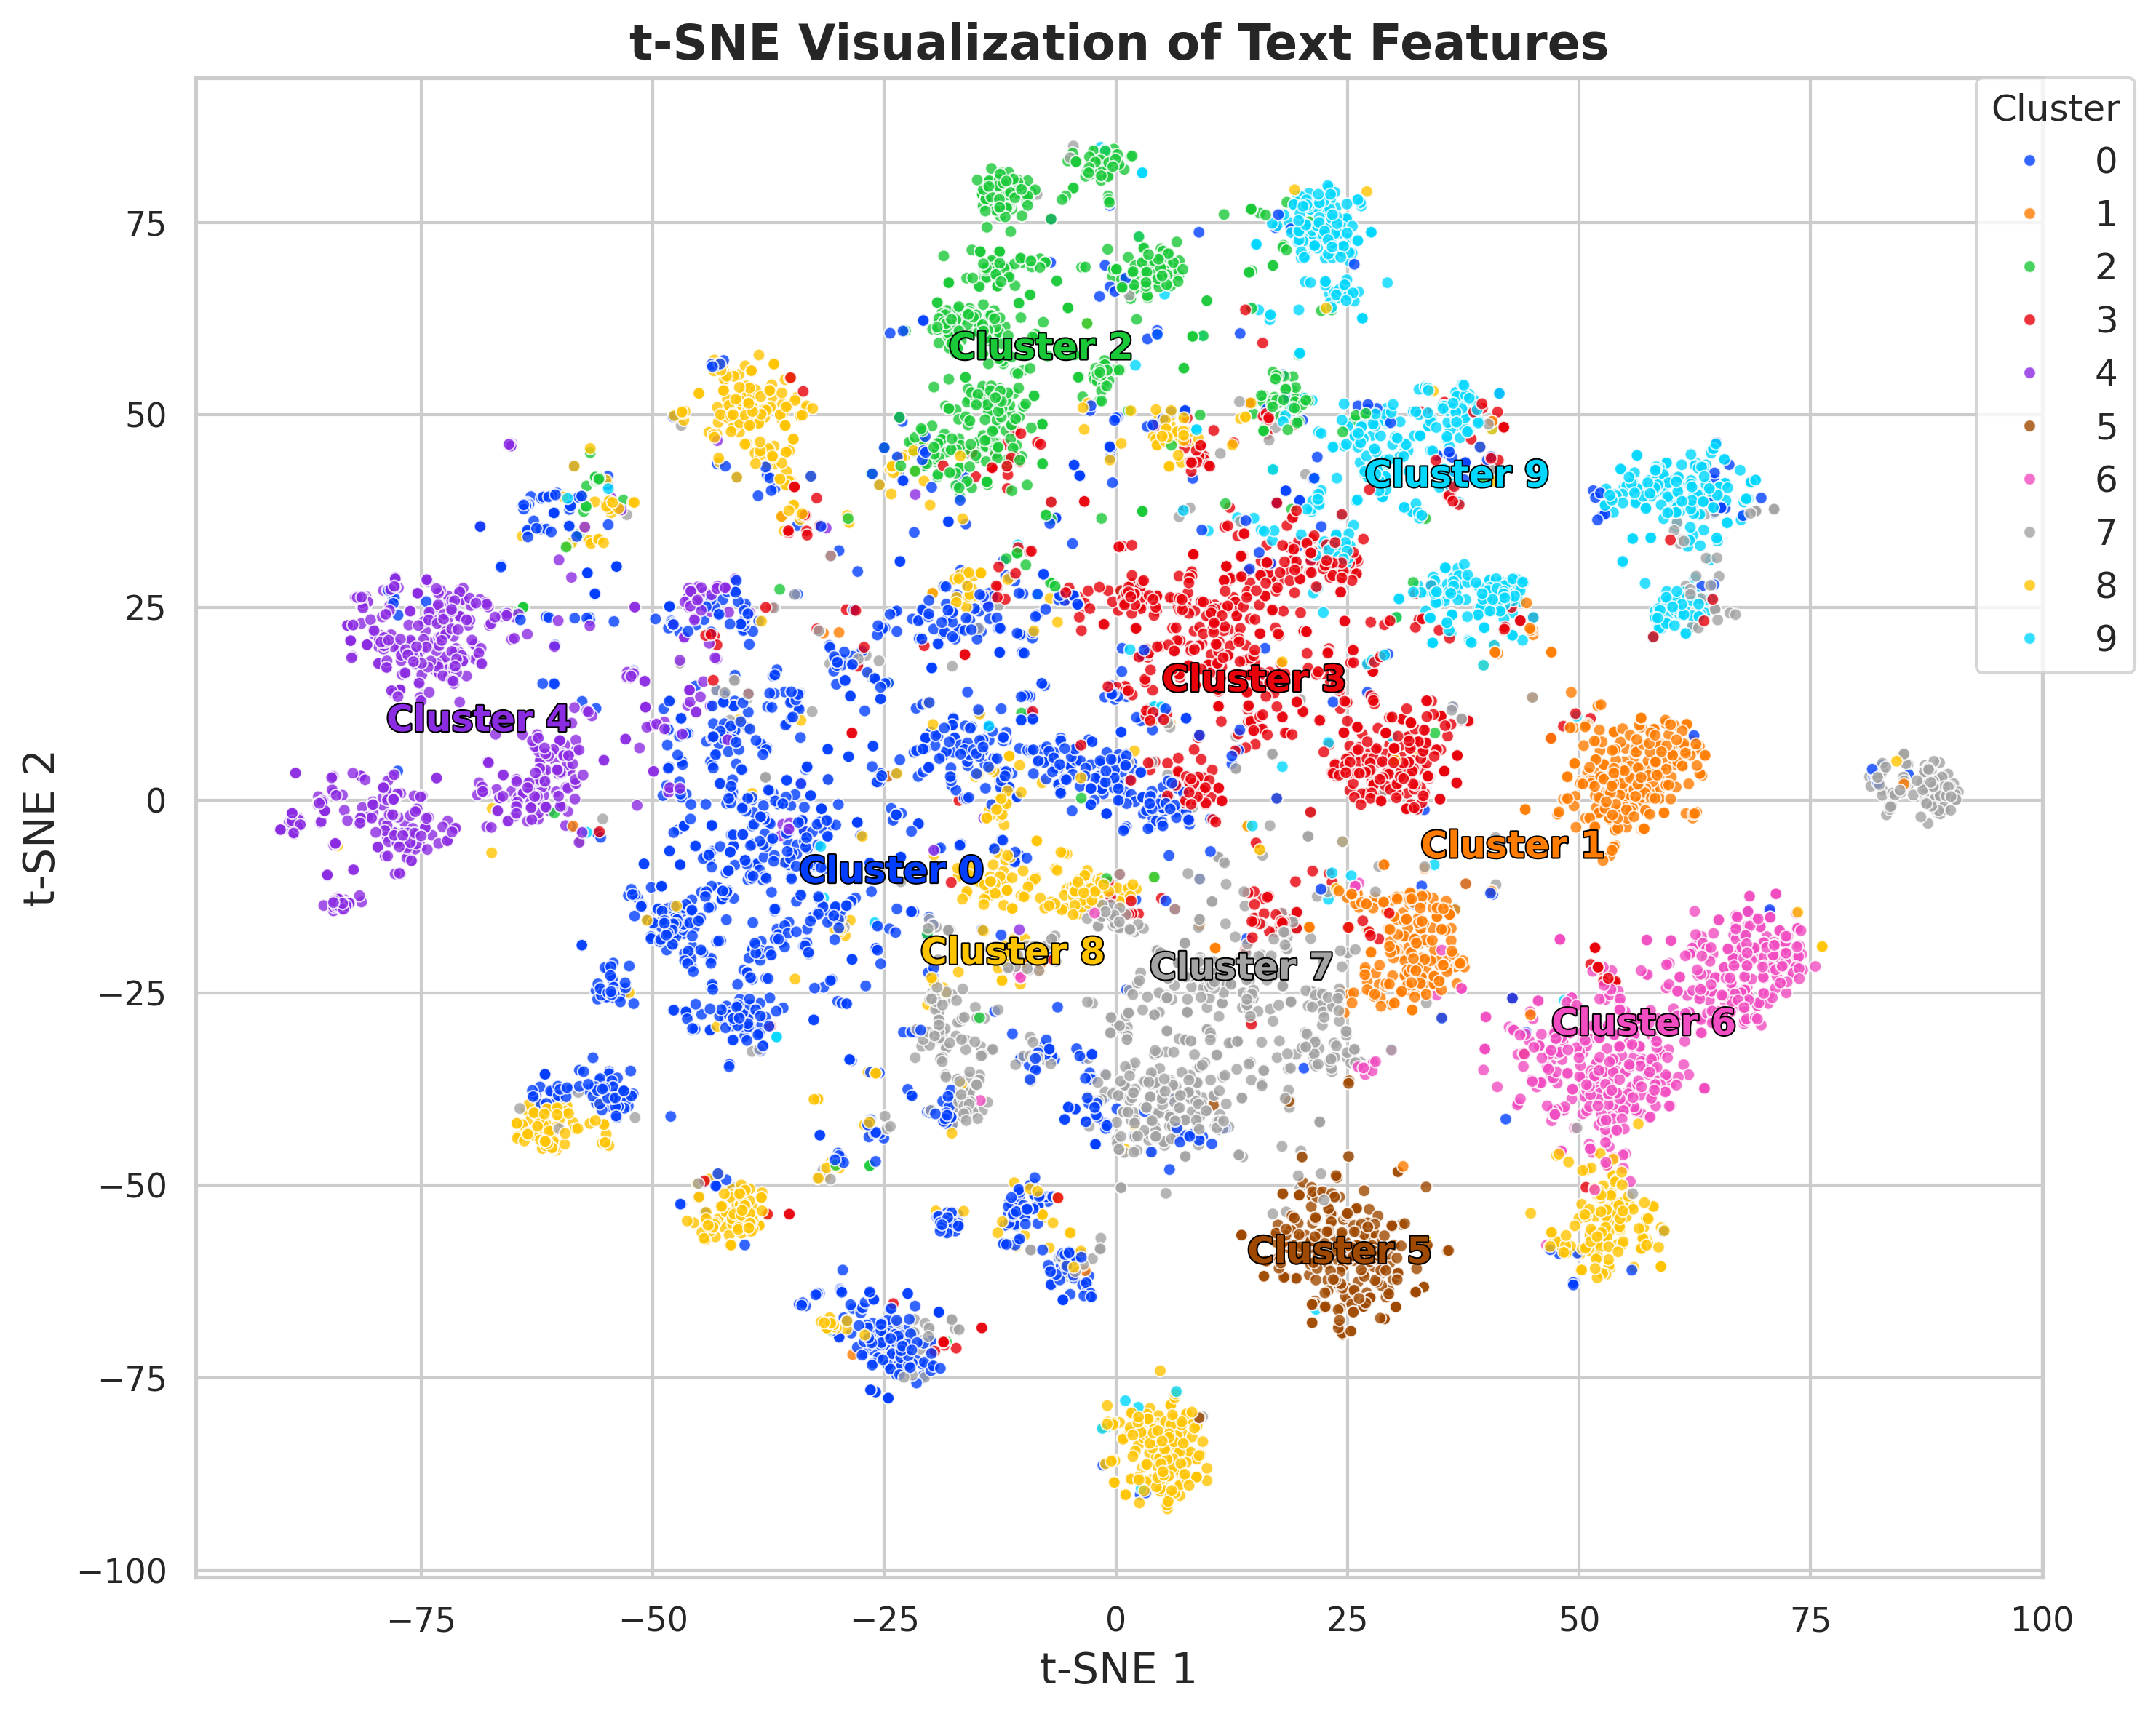
\includegraphics[width=0.3\textwidth]{figures/text_features/text_features_clusters_tsne_10.png}
  \caption{The figure shows a 2D t-SNE projection of text embeddings, revealing distinct clusters that capture meaningful semantic differences. The clusters demonstrate clear spatial separation.}
  \label{fig:text_feat_1}
\end{figure}
\subsection{Labeling dog and cat classes}
\begin{figure}[H]
  \centering
  \begin{minipage}{0.45\textwidth} % Adjusted width for the first image
    \centering
    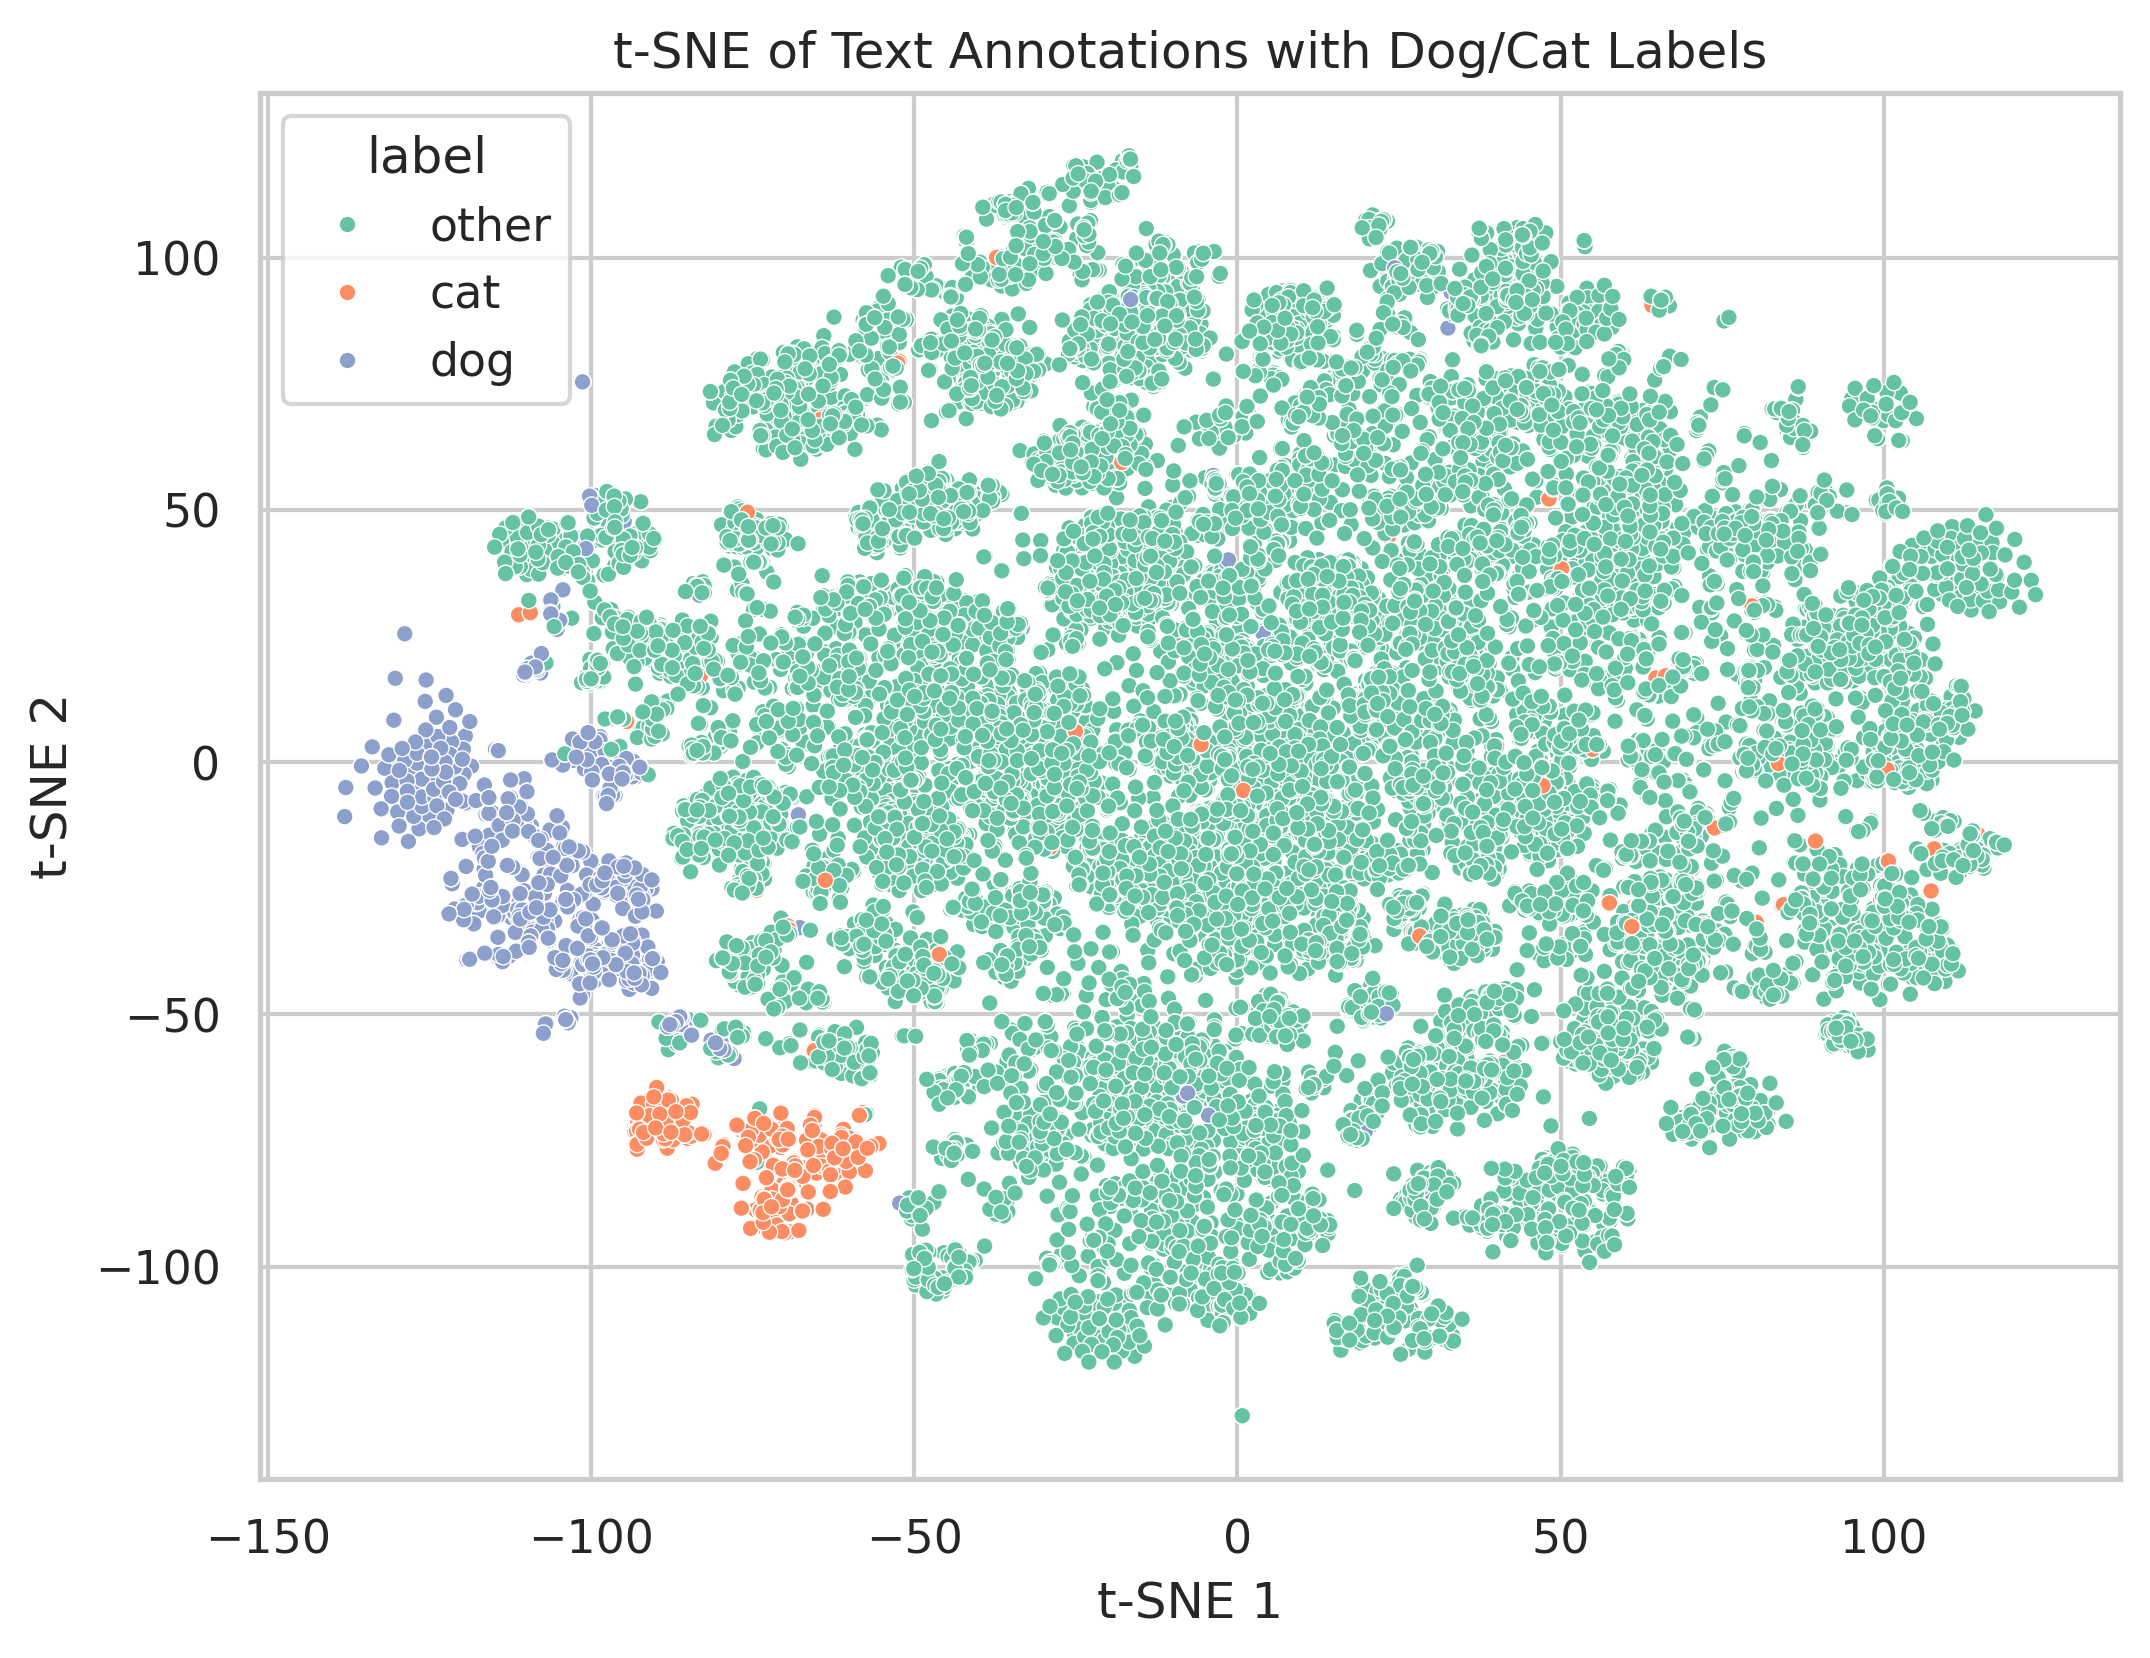
\includegraphics[width=0.5\linewidth]{figures/text_features/text_dogcat.png}
    \caption{The figure shows a t-SNE visualization of the "dog" and "cat" classes in the text embedding space, with well-separated and compact clusters.}
    \label{fig:silhouette_2}
  \end{minipage} \hspace{0.05\textwidth} % Horizontal space between the images
  \begin{minipage}{0.45\textwidth} % Adjusted width for the second image
    \centering
    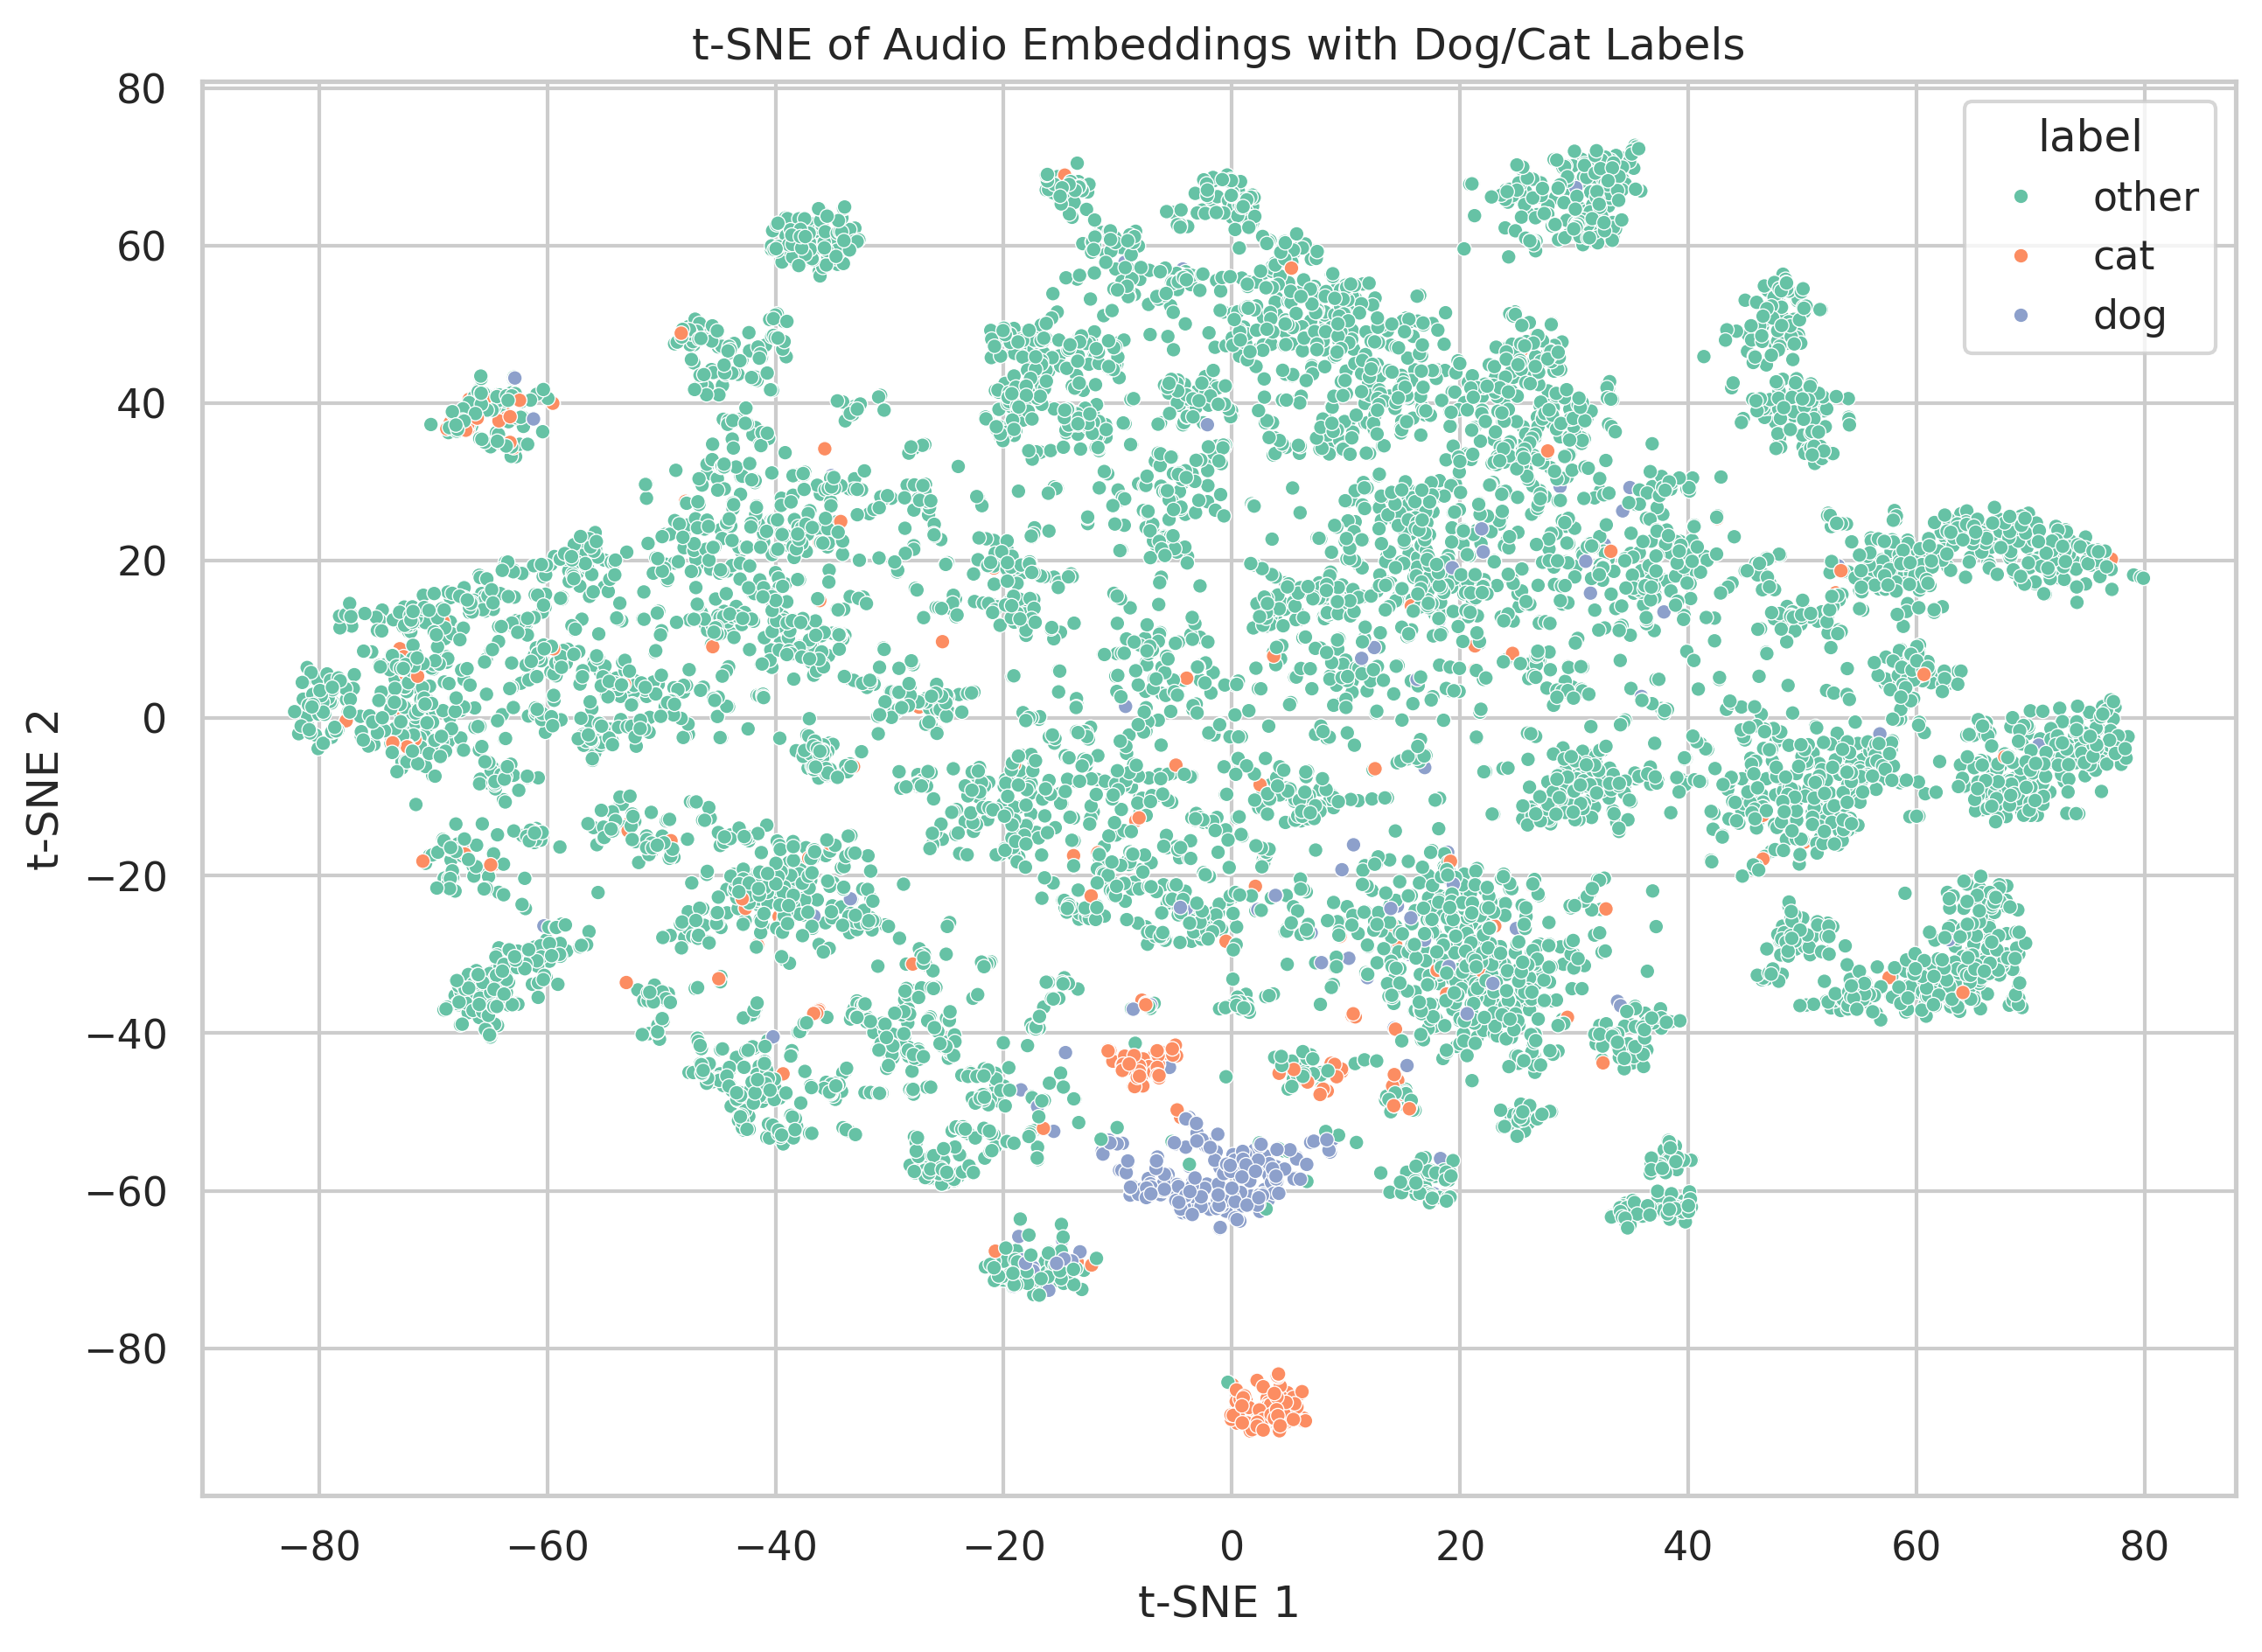
\includegraphics[width=0.5\linewidth]{figures/text_features/audio_dogcat.png}
    \caption{The figure shows a t-SNE visualization of the "dog" and "cat" classes in the audio embedding space, with overlapping and noisy clusters.}
    \label{fig:cluster_comp_2}
  \end{minipage}
\end{figure}

\subsection{Alignment of audio feature clusters with text clusters}

The text highlights a partial alignment between text and audio feature clusters in t-SNE visualizations (Figures 11 and 10). Specifically, Cluster 4 in the text plot (Figure 11) aligns with Cluster 2 in the audio plot (Figure 10), suggesting both modalities capture similar underlying semantics. While t-SNE may distort global structure, the local consistency of clusters indicates cross-modal similarities in data grouping.

\section{Conclusions}
\label{sec:conclusions}

The dataset offers strong potential due to its size and variety but has limitations for training general-purpose sound event detectors. Temporal annotations are mostly consistent, though some ambiguous segments could affect model accuracy. Textual annotations vary widely in wording, making it harder for models to reliably link sounds and text. Biases identified include annotation style, detail, outliers, and spelling errors, which highlight the need for careful training to ensure quality data is prioritized.
\end{document}
